\chapter{Exposici\'on del detector}
\label{ch:expAuger}

Para obtener la exposici\'on a neutrinos del detector es necesario integrar las eficiencias de identificaci\'on convolucionadas con la probabilidad de ocurrencia de los eventos considerados. Las eficiencias se derivan de los criterios de selecci\'on delineados en el cap\'itulo antecedente, donde se aplican en paralelo  a todos los procesos simulados para obtener, v\'ia integraci\'on, la exposici\'on combinada de los tres an\'alisis de neutrinos de Auger.
Por otro lado, las probabilidades de ocurrencia surgen de un an\'alisis del mecanismo de detecci\'on y, para el caso ES, del uso de simulaciones de Monte Carlo.
Para llevar a cabo la integraci\'on temporal y en \'area se utiliza una t\'ecnica que permite tener en cuenta las fluctuaciones del arreglo a trav\'es del tiempo donde, en particular, se desarroll\'o un m\'etodo para incluir el cambio en las eficiencias causado por el envejecimiento del detector.
Finalmente, se estudian en detalle las distintas fuentes de incertezas sistem\'aticas y se eval\'ua su contribuci\'on al resultado final.

% Finalmente, combinando la exposici\'on de los tres an\'alisis y sus errores sistem\'aticos se obtuvo la cota superior a la magnitud del flujo de neutrinos ultra energéticos m\'as estricta presentada por Auger hasta la fecha.

\section{C\'alculo de la exposici\'on}
\label{sc:expoNu}
	
	La exposición es una cantidad comunmente utilizada en física de astropartículas para caracterizar una medición.
	Se la define como la magnitud que, convolucionada con un flujo de partículas $\frac{dN_{\nu}}{d\gamma}$, resulta en la cantidad de eventos que se espera haber detectado durante la misma, y ser\'a simbolizada con la letra $\mathscr{E}$:
	%
	\begin{equation}
	 N_{esp}=\int\limits_{\Gamma}~\frac{dN_{\nu}}{d\gamma}~\mathscr{E}(\gamma) ~d\gamma
	 \label{eq:exp0}
	\end{equation}
	%
	aqu\'i, $\gamma$ simboliza el conjunto de variables del que dependa la detección, que en este trabajo corresponde a $(E_{\nu},\vec{r},\omega,t)$\footnote{Se desprecia cualquier tipo de inhomogeneidad en el flujo.}, es decir, la energía de los neutrinos incidentes, el punto en el que se realiza la medici\'on, el ángulo sólido que se observa y el tiempo durante el que se mide, respectivamente.
	
	De la ecuación \ref{eq:exp0} se desprende entonces que, como $\frac{dN_{\nu}}{d\gamma}$ es la cantidad de neutrinos de energía $E_{\nu}$ que alcanzan el detector por unidad de área, ángulo sólido y tiempo, la exposicion $\mathscr{E}(\gamma)=\mathscr{E}(E_{\nu},\vec{r},\omega,t)$ es la \emph{probabilidad} de detectar un neutrino con energia $E_\nu$ que incide en el punto $\vec{r}$ desde la direcci\'on $\omega$ en el instante $t$.
	La exposición entonces, contiene toda la información correspondiente a la medición y al detector, mientras que el flujo incluye la física de la fuente de lo que se espera detectar.
	
	Si se considera a $\frac{dN_{\nu}}{d\gamma}$ como un flujo difuso $\Phi(E_{\nu})$, es decir isótropo, homogeneo y constante en el tiempo, la ecuación \ref{eq:exp0} se escribe:
	%
	\begin{equation}
	 N_{esp}=\int\limits_{\mathbf{E_{\nu}}}~\Phi(E_{\nu})\left[~\iiint\limits_{T~\Omega~A}\mathscr{E}(E_{\nu},\vec{r},\omega,t) ~d\vec{r}~d\omega~dt~\right]~dE_\nu
	 \label{eq:exp1}
	\end{equation}
	%
	La función de $E_\nu$ entre corchetes, que corresponde a la exposición integrada en el caso de un flujo difuso, será llamada de aquí en más \emph{exposición del detector} y será simbolizada por la letra $\cal E$:
	%
	\begin{equation}
	 {\cal E}(E_\nu)\equiv\iiint\limits_{T~\Omega~A}\mathscr{E}(E_{\nu},\vec{r},\omega,t) ~d\vec{r}~d\omega~dt
	 \label{eq:exp2}
	\end{equation}
	%
	El objetivo a partir de aquí es la construcción de esta cantidad, que requiere de los siguientes ingredientes:
	\begin{enumerate}
	 \item La probabilidad de que un neutrino de energía $E_\nu$ proveniente de la direcci\'on  $\omega$~\footnote{Es decir, cuya dirección se caracteriza por los ángulos $(\theta,\phi)$.} de inicio a una lluvia atmosférica extendida de parámetros $\mathcal{X}$~\footnote{$\mathcal{X}$ es $(E_\tau,\omega,{\rm x_d})$ en ES y $(E_\nu,\omega,D)$ en DG.}.
	 \item La probabilidad de que una lluvia de parámetros $\mathcal{X}$ dispare el detector y que el evento registrado sea identificado como un neutrino, es decir, las eficiencias de identificación. Esta ser\'a adem\'as funci\'on de la posici\'on $\vec{r}$ y el instante $t$ en que sea detectada.
	 \item La integración de estas probabilidades sobre el área del detector, el tiempo de medición, las diferentes direcciones de arribo y las distintas lluvias atmosféricas que se puedan generar.
	\end{enumerate}
	
	Teniendo esto en cuenta, la ecuación \ref{eq:exp2} puede escribirse para DG y ES:
% 	%
% 	\begin{equation}
% 	 {\cal E}(E_\nu)\equiv\iiiint\limits_{T~\Omega~A~X}P(\mathcal{X}|E_{\nu},\vec{r},\omega,t)~\epsilon(\mathcal{X},\vec{r},t) ~d\mathcal{X}~d\vec{r}~d\omega~dt
% 	 \label{eq:exp3}
% 	\end{equation}
% 	% 
% 	Según lo discutido en la sección \ref{sc:libGen}, para eventos ES el parámetro $\mathcal{X}$ debe corresponder al conjunto $(E_\tau,{\rm x_d})$, mientras que en el caso de DG corresponde a la profundidad inclinada de interacción $D$.
% 	Por otro lado, la probabilidad de ocurrencia de un evento de parámetros $\mathcal{X}$ simplemente incluye la información del blanco con el que los neutrinos interactúan: la tierra en ES y la atmósfera en DG. 
% 	En ambos casos en este trabajo se desprecian las fluctuaciones que estos puedan tener durante el tiempo que dura la medición o al variar la fracción del detector que se esté estudiando (el punto $\vec{r}$), por lo que $P(\mathcal{X}|E_{\nu},\vec{r},\omega,t)~\rightarrow~P(\mathcal{X}|E_{\nu},\omega)$.
% 	Incuyendo toda esta información, para calcular la exposición del detector es necesario resolver las siguientes integrales:
% 	%
	\begin{equation}
	 {\cal E}_{DG}(E_\nu)\equiv\iint\limits_{\mathbf{D}~\Omega}P(D|E_{\nu},\omega)~
	 \left[~
	 \iint\limits_{T~A}\epsilon(E_{\nu},\omega,D,\vec{r},t)~d\vec{r}~dt
	 \right]
	 ~d\omega~dD
	 \label{eq:exp4DG}
	\end{equation}
	%
	y
	%
	\begin{equation}
	 {\cal E}_{ES}(E_\nu)\equiv\iiint\limits_{\mathbf{E_\tau}~\mathbf{x_d}~\Omega}P({\rm x_d},E_\tau|E_{\nu},\omega)~
	 \left[~
	 \iint\limits_{T~A}\epsilon(E_\tau,\omega,{\rm x_d},\vec{r},t)~d\vec{r}~dt
	 \right]
	 ~d\omega~d{\rm x_d}~dE_\tau
	 \label{eq:exp4ES}
	\end{equation}
	%
	
	Las siguientes secciones se dedican a la obtención de cada uno de los términos de estas integrales.
	
	\subsection{Término de probabilidad}
	
	El t\'ermino de probabilidad contiene la informaci\'on del blanco con el que interact\'uan los neutrinos. 
% 	
% 	El término de probabilidad conecta el flujo con las eficiencias en el cálculo de la exposición.
% 	En este caso, el flujo representa la cantidad de eventos que se esperan por unidad de área, tiempo y ángulo sólido, mientras que por construcción las eficiencias corresponden a la cantidad de eventos detectados segun variables relacionadas con el proceso de medición.
% 	Entonces, c
	Coloquialmente este responde a la prgunta: ¿qu\'e fracci\'on de los neutrinos que alcanzan el blanco iniciar\'an una EAS de par\'ametros $\mathcal{X}$?
	Cabe destacar que en este trabajo se desprecia cualquier fluctuaci\'on que suceda durante el tiempo $T$ en que se mide o al variar la fracción del detector que se esté estudiando, caracterizada por $\vec{r}$.
	
	
	\subsubsection{Eventos DG}
	
	Como se discuti\'o en la sección \ref{sbsc:easDG}, el camino libre medio de los neutrinos es varios órdenes de magnitud mayor que el espesor de la atmósfera, por lo que es una muy buena aproximacion considerar la probabilidad de interacción una constante para cualquier profundidad de interacción, o lo que es lo mismo, que la magnitud del flujo no depende de la misma.
	Con esto en mente, para obtener la expresión de $P(D|E_{\nu},\Omega)$ es útil primero considerar un caso simplificado: un haz de partículas caracterizado por un flujo de $F$ partículas por unidad de área y tiempo que incide sobre un blanco de $N$ part\'iculas. La cantidad de colisiones $n$ por unidad de tiempo viene dada por:
	%
	\begin{equation}
	% \frac{\Delta n}{\Delta t} 
	n = F\,\sigma\,N
	\label{eq:n1}
	\end{equation}
	% 
	donde $\sigma$ es la sección eficaz de interacción entre las part\'iculas del haz y del blanco.
	Si \'este \'ultimo, de masa $M$ se encuentra formado por elementos dispersores de masa $m$, \ref{eq:n1} queda:
	%
	\begin{equation}
	% \frac{\Delta n}{\Delta t} 
	n = F\,\sigma\,\frac{M}{m}
	\end{equation}
	% 

	Este resultado se puede extender para analizar el caso de un flujo diferencial difuso~$\Phi(E_{\nu})$ y un detector plano que registra todas las lluvias producidas por neutrinos que satisfacen las siguientes condiciones  (ver figura \ref{fig:diferencialMasa}):
	%
	\begin{itemize}
	\item su dirección de arribo apunta a una región $\Delta A$ del detector ubicada en $\vec{r}$
	\item su dirección de arribo $(\theta,\phi)$ está en un rango 
	$\Delta \Omega=\sen\theta\,\Delta\theta\,\Delta\phi$
	\item su energía~$E_{\nu}$ está en un rango $\Delta E_{\nu}$
	\item interactúa a una profundidad másica~$D$ en el rango $[D, D+\Delta D]$. 
	\end{itemize}
	%
	En este caso el número de lluvias observadas por unidad de tiempo está dado por:
	%
	\begin{equation}
	% \frac{\Delta \mathfrak{N}}{\Delta t}
	n = \Phi(E_{\nu})\, \Delta E_{\nu}\,\Delta\Omega\;\sigma(E_{\nu})\;\frac{\Delta M}{m}
	\label{eq:dn_domega}
	\end{equation}
	%
	donde la cantidad de masa $\Delta M$ contenida en un espesor $\Delta D $ depende del ángulo cenital, $\Delta M= \Delta D \, \Delta A \, \cos\theta$ (ver figura \ref{fig:diferencialMasa})\footnote{La profundidad másica $D$ tiene unidades de masa sobre área. Para el caso del Observatorio Auger, en Malarg\"ue, el espesor másico de la atmósfera vertical es de 860 g/cm$^2$.}.
	%  
	\begin{figure}[ht]
	\begin{center}$
	\begin{array}{cc}
	\includegraphics [width=0.52\textwidth]{fig/resultadosAuger/detectorPlano.pdf} & \includegraphics [width=0.42\textwidth]{fig/resultadosAuger/diferencialMasa.pdf}
	\end{array}$
	\end{center}
	\caption{
	\textit{Izquierdo}: esquema de un detector plano ideal (eficiencia 1), es decir, que mide todos los eventos producidos por partículas cuya dirección de arribo cruza su superficie. \textit{Derecha}: diferencial de masa $\Delta M$ para dos \'angulos cenitales. Se observa para $\Delta D$ fijo, $\Delta M$ disminuye al aumentar el ángulo cenital $\theta$.
	}
	\label{fig:diferencialMasa}
	\end{figure}
	%
	
	Si el detector en cambio tiene una eficiencia $\epsilon$ menor que uno, sólo una fracción de las lluvias serán detectadas. Agregando esta informaci\'on a la ecuaci\'on \ref{eq:dn_domega} y considerando el caso más general, en el que $\epsilon$ es función de $E_{\nu}$, $\theta$, $D$, $\vec{r}$, $t$ y $\phi$, se tiene:
	%
	\begin{equation}
	n = \frac{1}{m}\,\Phi(E_{\nu})\,\sigma(E_{\nu})\,\Delta E_{\nu}\,\Delta D\,\Delta A\,\cos\theta\sen\theta\,\Delta\theta\,\Delta\phi\;\epsilon(E_{\nu},\theta,D,\vec{r},\phi,t)
	\label{eq:dN_domega}
	\end{equation}
	%
	e integrando en $\phi$:
	%
	\begin{equation}
	n = \frac{1}{m}\,\Phi(E_{\nu})\,\sigma(E_{\nu})\,\Delta E_{\nu}\,\Delta D\,\Delta A\,\cos\theta\sen\theta\,\Delta\theta\,2\pi\;\epsilon(E_{\nu},\theta,D,\vec{r},t)
	\label{eq:dN_domega2}
	\end{equation}
	%
	donde $\epsilon(E_{\nu},\theta,D,\vec{r}) = \frac{1}{2\pi}\int \epsilon(E_{\nu},\theta,D,\vec{r},\phi)\,\d\phi$ es el promedio de la eficiencia respecto del ángulo azimutal. 

	Si se supone ahora que la medici\'on se extiende durante un tiempo $T$, pasando a forma integral y reacomodando la ecuación \ref{eq:dN_domega2} se obtiene:
	%
	\begin{equation}
	N = \int\limits_{\mathbf{E_\nu}}\Phi(E_{\nu})~
	\tilde{\cal E}_{DG}(E_{\nu})
	~dE_\nu
	\label{eq:dN_domega3}
	\end{equation}
	%
	donde $N=\int_{T} n dt$ y:
	%
	\begin{equation}
	\tilde{\cal E}_{DG}(E_{\nu})
	\equiv 2\pi\iint\limits_{\mathbf{D}~\Theta}\frac{1}{m}~\sigma(E_{\nu})\cos\theta
		\left[
			~\iint\limits_{T~A} \epsilon(E_{\nu},\theta,D,\vec{r},t)~d\vec{r}~dt
		\right]
		\sen\theta~d\theta~dD
	\label{eq:dN_domega4}
	\end{equation}
	
	Por otro lado, si se desarrolla el término $d\Omega$ y se integra en $\phi$ en la ecuación \ref{eq:exp4DG} se obtiene:
	\begin{equation}
	{\cal E}_{DG}(E_\nu)\equiv2\pi\iint\limits_{\mathbf{D}~\Theta}P(D|E_{\nu},\theta)~
	 \left[~
	 \iint\limits_{T~A}\epsilon(E_{\nu},\theta,D,\vec{r},t)~d\vec{r}~dt
	 \right]
	 \sen\theta~d\theta~dD
	\label{eq:exp5DG}
	\end{equation}
	
	Entonces, por comparación entre \ref{eq:dN_domega4} y \ref{eq:exp5DG} se tiene como se esperaba, que $P(D|E_{\nu},\theta)$ es una constante y vale:
	\begin{equation}
	 P(D|E_{\nu},\theta) = \frac{1}{m}~\sigma(E_{\nu})\cos\theta
	\end{equation}
	
	En este trabajo se utilizó la sección eficaz neutrino nucleón dada en \cite{cite:cooper_sarkar}.
	
	\subsubsection{Eventos ES}
	
	La expresión de este término en el caso de los eventos ES es algo mas complicada debido a que el proceso de detección consta de dos pasos:
	\begin{enumerate}
	 \item La primer interacción del \nutau{} dentro de la tierra y la propagación hasta el escape.
	 \item El decaimiento del \tauon{} en la atmósfera.
	\end{enumerate}
	
	En la sección \ref{sc:pesos} se analizó cada uno de estas etapas para corregir los pesos de las simulaciones de neutrinos ES.
	All\'i, la inclusión de la propagación dentro de la tierra se realizó mediante simulaciones de Monte Carlo (ver sección \ref{sbsbsc:sim_prop_tierra}).
	A partir de ellas se obtuvo el término $f(E_\tau|E_\nu,\theta)$, que representa la densidad de probabilidad de la energía de los \tauon{}'s que escapan de la tierra, si los neutrinos incidentes tienen energía \enu{} y ángulo cenital $\theta$.
	Por otro lado, la incorporación de la probabilidad de decaimiento del \tauon{} en la atmósfera también se analizó en la sección \ref{sc:pesos} y viene dada por la ecuación:
	%
	\begin{equation}
		h(x_d,(E_\tau,\theta))=
		\exp{\left(
		-\frac{x_d}{|\cos\theta|\lambda(E_\tau)}
		\right)}
		\frac{1}{|\cos\theta|\lambda(E_\tau)}
		\label{eq:h_xd}
	\end{equation}
	%
	Finalmente, es necesario incluir el término que tiene en cuenta la variación del diferencial de volumen en el que se produce la interacción con el ángulo cenital, $|\cos\theta|$.
	
	Con todo esto, desarrollando la integral en $\omega$ e integrando en $\phi$ la ecuación \ref{eq:exp4ES} queda:
	%
	\begin{equation}
	\begin{aligned}
	 {\cal E}_{ES}(E_\nu)\equiv2\pi\iiint\limits_{\mathbf{E_\tau}~\mathbf{x_d}~\Theta}P({\rm x_d},E_\tau|E_{\nu},\theta)~
	 \left[~
	 \iint\limits_{T~A}\epsilon(E_\tau,\theta,{\rm x_d},\vec{r},t)~d\vec{r}~dt
	 \right]\\
	 ~\sen\theta d\theta~d{\rm x_d}~dE_\tau
	 \end{aligned}
	 \label{eq:exp5ES}
	\end{equation}
	%
	donde:
	\begin{equation}
	 P({\rm x_d},E_\tau|E_{\nu},\theta)=
	 f(E_\tau|E_\nu,\theta)
	 h({\rm x_d},(E_\tau,\theta))
	 |\cos\theta|
	 \label{eq:exp5.2ES}
	\end{equation}
	
	\subsection{Eficiencias de identificación en un detector infinito}
	\label{sbsc:idealEff}
	
	Para construir las eficiencias en un detector real es útil estidiarlas antes sobre un detector ideal.
	Mientras que el detector real no s\'olo es finito sino que su forma cambia en el tiempo, por ejemplo debido a estaciones que entran y salen de servicio, un detector ideal consiste en una representación infinita, regular y constante del verdadero.
	Entonces, para obtener las eficiencias de identificación de cada uno de los análisis se simuló una copia del SD de Auger de \cant{50\times50}{km}, infinita a los fines prácticos\footnote{La huella de part\'iculas de los eventos simulados no suelen los \cant{25}{km} de extensión. Adem\'as, ser\'ia extremadamente raro que considerar el excedente de part\'iculas en un evento de tal tama\~no modifique la condici\'on de trigger e identificaci\'on.}, se lanzó sobre su centro las lluvias simuladas y se obtuvo la señal en el detector tal como se explicó en la sección \ref{sc:offline}.
	Luego, se aplicaron los criterios de identificación de neutrinos desarrollados en el capítulo \ref{ch:selAuger} y se calculó la eficiencia en cada bin con la siguiente ecuación:
	%
	\begin{equation}
	 \epsilon_\eta(\mathcal{X})=\frac{N_{\eta}(\mathcal{X})}{N_{sim}(\mathcal{X})}
	 \label{eq:effDef}
	\end{equation}
	%
	donde $\mathcal{X}$ es la etiqueta del bin, mientras que $N_{\eta}$ y $N_{sim}$ son la cantidad de lluvias que se identificaron con el criterio $\eta$ y simularon en el mismo. En nuestro análisis $\eta$ puede representar el nivel de disparo T3 del detector, la clasificación de  evento inclinado y la identificación como neutrino.
	
	\subsubsection{Eficiencias a neutrinos DG}
	
	La eficiencia a neutrinos DG depende de los siguientes parámetros:
	%
	\begin{itemize}
	 \item la profundidad de interacción $D$
	 \item el ángulo cenital $\theta$
	 \item la energía del neutrino $E_\nu$
	 \item sabor del neutrino $(e,\mu,\tau)$
	 \item tipo de interacción (CC o CN)
	\end{itemize}
	%
	Si bien esta también podría depender del ángulo azimutal $\phi$, al haber sido simulado de manera aleatoria, la eficiencia obtenida en cada bin de $(E_\nu,\theta,D)$ y para cada sabor y canal de interacción, representa el promedio en el ángulo azimutal.
	A partir de aqu\'i se detalla como var\'ian las eficiencias de disparo e identificaci\'on con los diferentes par\'ametros de los que depende.
	
	Para mostrar el comportamiento como funci\'on de la profundidad de interacci\'on $D$, la figura \ref{fig:effDG_tr_id} muestra la eficiencia de disparo T3 e identificación como función de esta variable para lluvias iniciadas por $\nu_e$ via CC, con \cant{E_\nu=10^{19}}{eV} y $\theta=85^\circ$.
	%
	\begin{figure}[ht!]
		\begin{center}
			\includegraphics[width=0.7\textwidth]{fig/resultadosAuger/eff_10EeV_85}
			\caption{Eficiencia de disparo T3 e identificación en función de la profundidad de interacción para lluvias iniciadas por $\nu_e$ via CC con \cant{E_\nu=10^{19}}{eV} y $\theta=85^\circ$}
			\label{fig:effDG_tr_id}
		\end{center}
	\end{figure} 
	%
	En estas condiciones existe un conjunto de profundidades a las que la eficiencia de disparo e identificaci\'on pr\'acticamente saturan. 
	Sin embargo, cuando la lluvia se inicia cerca de los \cant{3000}{g\,cm^{-2}}~\footnote{La profundidad a este \'angulo es cercana a los \cant{10000}{g\,cm^{-2}}}, aunque logra disparar el detector en alrededor del $70\%$ de los casos, la eficiencia de identificaci\'on se anula.
	Esto se debe a que la componente electromagn\'etica se agota luego de \cant{\sim2500}{g\,cm^{-2}} y los eventos generados no pueden ser distinguidos de los iniciados por hadrones.
	Por otra parte, cuando la lluvia se inicia muy cerca del detector no alcanza a evolucionar lateralmente lo suficiente como para disparar tres o mas estaciones, provocando menos eventos detectados. 
	
	La figura \ref{fig:effDG_en} se muestran las eficiencias para lluvias iniciadas por $\nu_e$ via CC con \cant{\theta=85}{^\circ} y \cant{E_\nu=10^{17},~10^{18},~10^{19}}{eV}.
	Naturalmente, dado que la cantidad de partículas que se generan en la lluvia es proporcional a la energía del primario, la eficiencia de detección aumenta con la misma.
	No obstante, las bajas energías son relativamente importantes en el cálculo de la exposición dado que los modelos cosmog\'enicos actuales predicen un flujo del tipo $E_\nu^{-2}$.
	%
	\begin{figure}[ht!]
		\begin{center}
			\includegraphics[width=0.7\textwidth]{fig/resultadosAuger/eff_varios_85}
			\caption{Eficiencia de identificación en función de la profundidad de interacción para lluvias iniciadas por $\nu_e$ via CC y por $\nu_x$ via CN para varias energías y \cant{\theta=85}{^\circ}}
			\label{fig:effDG_en}
		\end{center}
	\end{figure}
	%
	
	En la figura \ref{fig:effDG_th} se muestra como ejemplo las eficiencias de disparo e identificación para $\nu_e$ via CC y \cant{E_\nu=10^{18}}{eV} para \cant{\theta=80}{^\circ} en el panel izquierdo y para \cant{\theta=85}{^\circ} en el derecho.
	%
	\begin{figure}[ht!]
		\begin{center}
			\includegraphics[width=0.47\textwidth]{fig/resultadosAuger/eff_1EeV_80}
			\hfill
			\includegraphics[width=0.47\textwidth]{fig/resultadosAuger/eff_1EeV_85}
			\caption{El panel izquierdo (derecho) muestra las eficiencias de disparo T3, de selección de eventos inclinados y de indentificación como función de la profundidad medida desde el detector para neutrinos con \cant{\theta=80}{^\circ} (\cant{\theta=85}{^\circ}). Es posible observar que la eficiencia alcanzada por el discriminante de fisher es alta para ambos ángulos.}
			\label{fig:effDG_th}
		\end{center}
	\end{figure}
	%
	En el panel izquierdo (\cant{\theta=80}{^\circ}) la eficiencia de disparo T3 alcanza el 100$\%$ a profundidades intermedias mientras que la eficiencia de identificación máxima es cercana a 60$\%$.
	Esta diferencia es producida por los cortes de selección de calidad, en los que para el canal DGH (al que corresponden estos ángulos) se requieren al menos 4 estaciones con disparo local T2, cuando el disparo global T3 requiere sólo 3.
	El panel derecho de la misma figura muestra las mismas eficiencias para \cant{\theta=85}{^\circ}, y se observa que la identificación alcanza valores cercanos a 95$\%$.
	Esta ganancia se debe a un efecto puramente geométrico, ya que la longitud de la huella sobre el detector crece con un factor aproximadamente $1/\cos\theta$, tal como se esquematiza en la figura \ref{fig:effDG_th_sktch}.
	%
	\begin{figure}[ht!]
		\begin{center}
			\includegraphics[width=0.7\textwidth]{fig/resultadosAuger/huellas}
			\caption{La cantidad promedio de estaciones disparadas por evento aumenta con el ángulo cenital $theta$ debido a que la huella de las llubias sobre el detector crece aproximadamente con un factor $1/\cos\theta$.}
			\label{fig:effDG_th_sktch}
		\end{center}
	\end{figure}
	%
	
	Otra particularidad de los neutrinos DG es que hay que hacer distinción entre los distintos sabores de neutrino y los canales de CC y CN.
	Dado que tanto en CN como en CC $\nu_\mu$ la energía transmitida a la lluvia es en promedio del 20$\%$ de la energía del neutrino, la eficiencia de estos canales será menor que el caso CC $\nu_e$, tal como se observa en el panel izquierdo de la figura \ref{fig:effDG_cc_nc}.
	%
	\begin{figure}[ht!]
		\begin{center}
			\includegraphics[width=0.47\textwidth]{fig/resultadosAuger/eff_CCvsNC_85}
			\hfill
			\includegraphics[width=0.47\textwidth]{fig/resultadosAuger/eff_tau_1EeV_85}
			\caption{Eficiencia de identificación en función de la profundidad de interacción para lluvias iniciadas por $\nu_e$ via CC y por $\nu_x$ via CN con \cant{10^{18}}{eV} y \cant{85}{^\circ}}
			\label{fig:effDG_cc_nc}
		\end{center}
	\end{figure}
	%
	El panel derecho de la misma se observa para los mismos parámetros la comparación entre el canal de CN y CC via $\nu_\tau$.
	En la sección \ref{sbsc:easDG} se explicó el mecanismo DB, en el que un $\nu_\tau$ interactua via CC produciendo un lepton $\tau$ que puede decaer generando una segunda lluvia a algunos km de la primer interacción.
	Teniendo en cuenta que la transferencia de energía $\nu$-nucleón no depende de si la interacción es via CC o CN, se deduce de la figura que incluso cuando la cascada generada en la primer interacción no es suficiente para disparar el detector (para profundidades mayores a \cant{\sim2000}{g cm^{-2}}) la segunda cascada a veces lo hace, recuperando del orden del 10$\%$ de los eventos.
	
	\subsubsection{Eficiencias a neutrinos ES}
	
	La eficiencia a neutrinos ES depende de los siguientes parámetros:
	%
	\begin{itemize}
	 \item la energía del tauón $E_\tau$
	 \item la altura a la que decae $x_d$
	 \item el ángulo cenital $\theta$
	\end{itemize}
	%
	En este caso, dado que tanto el canal de decaimiento del tauón y la energía acarreada por sus productos, como el ángulo azimutal $\phi$ se simularon de manera aleatorea, la eficiencia obtenida en cada bin de $(E_\tau,x_d,\theta)$ será un promedio sobre el ángulo azimutal y las maneras de decaer del tauón.
	
	En la figura \ref{fig:effES_tr_id} se muestra a modo de ejemplo la eficiencia de disparo T3 y de identificación como función de la altura de decaimiento $\rm x_d$ para una energía de \cant{E_\tau=1}{EeV} y un ángulo cenital $\theta=90.68^\circ$.
	%
	\begin{figure}[ht!]
		\begin{center}
			\includegraphics[width=0.7\textwidth]{fig/resultadosAuger/eff_18_8931_forThesis}
			\caption{Eficiencia de disparo T3 e identificación en función de la altura de decaimiento del tauón para \cant{E_\tau=1}{EeV} y $\theta=90.68^\circ$. La línea horizontal marca la máxima eficiencia posible debido al canal a $\mu\nu_\mu\nu_\tau$ mientras que la línea vertical señala la altura de decaimiento típica a esta energía y ángulo (ver texto).}
			\label{fig:effES_tr_id}
		\end{center}
	\end{figure}
	%
	Se observa que el criterio de identificación de neutrinos ES selecciona la mayoría de los eventos que logran disparar el detector.
	También, por debajo de \cant{{\rm x_d}=300}{m} tanto la eficiencia de disparo como la de identificación alcanzan el máximo valor posile, que no puede exceder 0.822 debido a que el canal a $\mu\nu_\mu\nu_\tau$ no da lluvias detectables.
	Este valor se señala con una línea horizontal punteada.
	
	Por encima de \cant{{\rm x_d}=300}{m} la eficiencia decrece con ${\rm x_d}$ debido a que cada vez menos partículas alcanzan el detector.
	Sin embargo, la altura característica de decaimiento para \cant{E_\tau=1}{EeV} y $\theta=90.68^\circ$ es $\lambda_h = \lambda_D\times\cos(\pi - \theta) = 4.9{\rm km} \times 0.0119 = 580{\rm m}$, como se indica con una líena punteada vertical.
	Esto quiere decir que, como se detectan eventos hasta \cant{x_d\sim800}{m}, el $75\%$ de los $\tau$'s decaerán a alturas con eficiencia de decaimiento mayor a cero.
	
	En la figura \ref{fig:effES_en} se grafica la eficiencia de identificación para \cant{E_\tau=10^{17.5},~E_\tau=10^{18},~E_\tau=10^{18.5}}{eV}.
	Como era de esperarse, existe un incremento en la eficiencia con la energía, producto de la mayor cantidad de partículas generada durante la evolución de la lluvia, que aumenta las chances de disparar más estaciones.
	%
	\begin{figure}[ht!]
		\begin{center}
			\includegraphics[width=0.7\textwidth]{fig/resultadosAuger/eff_multEnergy_forThesis}
			\caption{Eficiencia de disparo T3 e identificación en función de la altura de decaimiento del tauón para $\theta=90.68^\circ$ y diferentes energías. Las líneas verticales señalan la altura de decaimiento típica del tauón:\cant{185}{m} (\cant{E_\tau=10^{17.5}}{eV}), \cant{580}{m} (\cant{E_\tau=10^{18}}{eV}) y \cant{1850}{m} (\cant{E_\tau=10^{18.5}}{eV}).}
			\label{fig:effES_en}
		\end{center}
	\end{figure}
	%
	Por un lado, cuando el decaimiento se produce cerca del suelo (valores ${\rm x_d}$ bajos) la eficiencia crece hasta alcanzar su valor máximo, 0.822.
	Por otro, a energías más altas se extiende el rango de ${\rm x_d}$ con eficiencia no nula.
	Cabe destacar aunque la eficiencia crezca con la energía, la altura de decaimiento típica lo hace de manera mucho más pronunciada (directamente proporcional a la energía), por ende, en resumen, el porcentaje de eventos detectados como función de la energía decrece.
	Esto puede observarse en la figura \ref{fig:effES_en}, en la que se marca con l\'ineas verticales la altura de decaimiento típica de cada energía. 
	
	Otro aspecto interesante de las eficiencias a neutrinos ES reside en su dependencia con el ángulo cenital.
	Como puede observarse en la figura \ref{fig:effES_th} la eficiencia decrece a medida que el tauón emerge de la tierra mas verticalmente.
	Esto se entiende debido a que las partículas del frente de la lluvia tendrán menos chances de alcanzar el suelo debido a que su dirección de propagación, en promedio, será también más vertical.
	Por otro lado, la altura de decaimiento característica del tauón depende del ángulo cenital según $\lambda_h=\lambda_D\times\cos(\pi-\theta)$, por lo que a energía fija ($\lambda_D$ fijo), la fracción de eventos detectados decrece rápidamente con el ángulo.
	Por ejemplo, para los 3 ángulos cenitales que se muestran en la figura \ref{fig:effES_th} la fracción de tauones que decaen a alturas en las que la eficiencia de identificación es 0 es 0.21 a $\theta=90.68^\circ$, 0.68 a $\theta=91.83^\circ$ y 0.85 a $\theta=92.98^\circ$.
	%
	\begin{figure}[ht!]
		\begin{center}
			\includegraphics[width=0.47\textwidth]{fig/resultadosAuger/eff_multiTheta_forThesis}
			\hfill
			\includegraphics[width=0.47\textwidth]{fig/resultadosAuger/eff_multTheta_h10_forThesis}
			\caption{Izquierda: eficiencia de identificación como función de la altura de decaimiento del tauón con energía \cant{E_\tau=10^{18}}{eV} y varios ángulos cenitales. La líena vertical a \cant{x_d=580}{m} marca la altura típica del decaimiento para $\theta=90.68^\circ$. Para $\theta=91.83^\circ$ y $\theta=92.98^\circ$ las alturas típicas de decaimiento son 1560 y \cant{2540}{m}, fuera de escala.
			Derecha: Las mismas eficiencias pero como función del parámetro $h_{10}$ (ver texto).}
			\label{fig:effES_th}
		\end{center}
	\end{figure}
	%
	
	Es muy interesante introducir la variable $h_{10}\equiv x_d + 10{\rm km} \times\cos(\pi-\theta)$, que corresponde a la altitud del eje de la lluvia a \cant{10}{km} del decaimiento del tauón.
	En el panel derecho de la figura \ref{fig:effES_th} se uestra la eficiencia como función de $h_{10}$ para los 3 ángulos cenitales.
	Puede observarse como a primer orden, la eficiencia de identificación no depende de $\theta$ y ${\rm x_d}$ por separado sino de $h_{10}$.
	Esto se debe a que al tratarse de eventos muy horizontales, la probabilidad de detección depende básicamente de la altura a la que se alcanza el máximo desarrollo de la lluvia \cite{cite:tesisYann}.
	Para las energías consideradas en este análisis, este máximo se produce aproximadamente a \cant{10}{km} del decaimiento del tauón.
	En particular, la figura \ref{fig:effES_th} muestra que es altamente improbable detectar un evento iniciado por un tauón de \cant{E_\tau=10^{18}}{eV} cuyo máximo se produce a más de \cant{1000}{m} sobre detector.
	 
	
	\subsection{Integración de las eficiencias sobre el área del detector}
	
	Para llevar a cabo la integración en área de la ecuación \ref{eq:exp2} es necesario estudiar cómo varían las eficiencias cuando se considera un detector finito, es decir, con bordes.
	Cuando una lluvia cae sobre una región completamente instrumentada del detector (interior y sin estaciones faltantes) la eficiencia será la ideal, calculada en la sección \ref{sbsc:idealEff}.
	Sin embargo, existen casos en los que el baricentro de las partículas de la lluvia puede caer hasta una decena de kilómetros fuera del detector y aun así disparar suficientes estaciones como para que el evento sea identificado como neutrino. 
	Esto se esquematiza en la figura \ref{fig:lluviaFuera} para neutrinos DG y ES.
	%
	\begin{figure}[ht!]
		\begin{center}
			\includegraphics[width=0.8\textwidth]{fig/resultadosAuger/lluviaFuera}\\
			\vspace*{0.1\textwidth}
			\includegraphics[width=0.8\textwidth]{fig/resultadosAuger/lluviaFuera_ES}
			\caption{Arriba (Abajo): esquema de una lluvia DG (ES) que se desarrolla fuera del \'area instrumentada e interact\'ua parcialmente con el detector. En ciertos casos este tipo de eventos pueden alcanzar un nivel de disparo T3.}
			\label{fig:lluviaFuera}
		\end{center}
	\end{figure}
	%
	
	En este contexto, se define un área circular extendida que contiene al detector finito y es suficientemente grande como para contemplar la contribución de las lluvias cuyo punto de impacto $\vec{r}$ cae fuera del detector\footnote{En otras palabras, el tamaño del círculo se selecciona tal que las lluvias que caen fuera del mismo tengan una probabilidad nula de disparar el detector.} (ver figura \ref{fig:aperturaReal}).
	
	Realizar la integral en área de la eficiencia consiste en hallar la eficiencia de identificación promedio en el área circular extendida~$A$.
	%
	\begin{equation}
	\langle\epsilon(\mathcal{X},t)\rangle_{\rm A} \equiv \epsilon(\mathcal{X}) =
	\frac{1}{A}
	\int\limits_{A}\!\epsilon(\mathcal{X},\vec{r},t)\,d\vec{r}
	\end{equation}
	%
% 	Esta eficiencia depende de la cantidad y distribución espacial (configuración) de las estaciones de superficie que conforman al detector finito que se está considerando.
	Es importante notar que si bien $\epsilon(\mathcal{X})$ depende de la elección del área extendida $A$\footnote{Naturalmente la eficiencia cae al aumentar el \'area sobre la que se tiran las lluvias.}, su producto $\epsilon(\mathcal{X})\times A$ es una constante intrínseca del detector llamada área efectiva $A_{\rm ef}$:
	%
	\begin{equation}
	A_{\rm ef}(\mathcal{X},t)=\int\limits_{A}\!\epsilon(\mathcal{X},\vec{r},t)\,d\vec{r}
	\label{eq:Aeff}
	\end{equation}
	%
	y representa la superficie de un detector equivalente 100\% eficiente.
	
	Para calcular esta magnitud se podría en principio realizar la integraci\'on para cada configuración por la que haya pasado el detector durante la medici\'on.
	Sin embargo, este camino es impráctico y requeriría un volumen de cómputo inaceptable.
	Por esta razón, se tom\'o un enfoque diferente que permite reusar las simulaciones producidas, sobre ciertas configuraciones representativas del detector.
	Para cada una el procedimiento es el siguiente:
	\begin{enumerate}
	 \item Los puntos de impacto $\vec{r}$ de las lluvias simuladas sobre un arreglo ideal son ubicados al azar dentro de la circunferencia del área extendida\footnote{En eventos ES lo que se ubica es el baricentro energ\'etico de las part\'iculas de la huella.}.
	 \item Las estaciones de los eventos simulados sobre el arreglo infinito que no coinciden con una estación activa del arreglo finito son descartadas del evento (ver figura \ref{fig:aperturaReal}).
	 \item Se reevalúan las condiciones de trigger T3 y, en caso de que se satisfagan, se recomputan las variables globales, los cortes de selección de lluvias inclinadas y lluvias jóvenes.
	\end{enumerate}

	En la figura \ref{fig:aperturaReal} se resume, a modo de ejemplo, los resultados posibles de reevaluar un evento que se identifica como neutrino sobre un arreglo infinito.
	
% 	El cociente de eventos identificados sobre eventos totales, determina la eficiencia de identificación promedio $\epsilon(E_\nu,\theta,D)$ de la configuración:
% %
% \begin{equation}
% \epsilon (E_\nu, \theta, D) = \frac{N_{\rm id}(E_\nu, \theta, D)}{N_{\rm sim}(E_\nu, \theta, D)} 
% \end{equation}
% %
% El $A_{\rm ef}(E_\nu,\theta,D,t)$ se obtiene multiplicando este valor por la superficie del área extendida $A$.
	
	%
	\begin{figure}[ht!]
		\begin{center}
			\includegraphics[width=0.63\textwidth]{fig/resultadosAuger/aperturaReal}
			\caption{Ejemplo del resultado de ubicar la misma lluvia, iniciada por un neutrino profundo, en cuatro posiciones diferentes, sobre una configuración dada del detector.
			Las flechas indican la dirección de avance de la lluvia, los puntos representan el arreglo ideal e infinito de estaciones y la circunferencia el área de detección extendida (ver texto).
			Los símbolos sólidos corresponden a estaciones de la lluvia simulada que presentan trigger T2 y que también están activas en la configuración de referencia.
			Los símbolos abiertos indican estaciones que no se encuentran en el arreglo real. Los símbolos redondos indican las lluvias identificadas como neutrinos y los cuadrados las que no.
			En el caso~1 la lluvia está completamente contenida y es identificada como neutrino. En~2 cae completamente fuera de la configuración de referencia y, por lo tanto, no produce T3 sobre el detector real.
			Aunque en el caso~3 la lluvia está parcialmente contenida y dispara el SD, no es identificada como neutrino debido a que sus estaciones tempranas no son registradas en el detector real. En~4, la lluvia pierde sus estaciones tardías pero es aún identificada ya que conserva su región temprana que es la que más influye en la discriminación.}
			\label{fig:aperturaReal}
		\end{center}
	\end{figure}
	%
% 	\clearpage
	
	\subsection{Integración temporal: evolución del detector}
	
	Incluir la evolución temporal del detector en la integración de la ecuación \ref{eq:exp2} no es simple.
	Si bien la construcción del SD de Auger concluyó a finales de 2008, y se comporta de manera estable desde entonces, es común que algunas estaciones salgan de servicio temporalmente por mantenimiento, fallas o situaciones fortuitas.
	Por este motivo el estado del detector es monitoreado cada segundo mediante la frecuencia de disparo T2 de todas las estaciones.
	A partir de esta información se generan archivos que registran las configuraciones (conjunto de estaciones activas) del SD con una resolución de un segundo.
	
	Entonces, de manera ideal, habría que evaluar la exposición de todas las configuraciones por las que pasa el detector y realizar la integración mediante una suma pesada por la cantidad de tiempo que se mantiene en cada una.
	Como no es posible procesar tal cantidad de información, se dividió el periodo de búsqueda en intervalos de 3 días y se tomó, para cada uno de ellos, una configuración representativa. 
	Luego, a cada una de estas configuraciones se le asignó un peso determinado por la fracción del tiempo en que el detector se encuentra en dicha configuración representativa, o en una de mayor eficiencia dentro de dicho intervalo.
	
	Para cada periodo de tiempo, no es evidente cual de las configuraciones por las que pasa el SD es conveniente elegir.
	Para abordar este problema se trabajó bajo la aproximación de que, dentro de los 3 días de duración del periodo, la exposición es una función de la cantidad de estaciones activas y no de su distribución espacial particular.
	Si bien es claro que esta aproximación no es válida en general\footnote{Por ejemplo, a misma cantidad de estaciones, una fila de estaciones no tiene la misma exposición que un arreglo cuadrado}, es muy buena al restringirse a periodos de tiempo lo suficientemente cortos tal que las configuraciones, con muchas estaciones activas, por las que pasa el detector son muy similares.
	
	En la figura \ref{fig:t2FilePlot} se muestra, a modo de ejemplo, la cantidad de estaciones activas en función del tiempo para el periodo que va del 3/01/08 al 5/01/08. Las zonas sombreadas corresponden a periodos, conocidos como ``bad periods", en los que el detector se encontraba particularmente inestable y que son removidos del análisis.
	Como puede verse, la cantidad de estaciones activas es esencialmente constante la mayor parte del tiempo con la excepción de breves periodos en los que puede caer significativamente.
	En estos intervalos la configuración espacial del detector puede ser significativamente diferente y la aproximación de que la exposición depende solo del número de estaciones deja de ser válida.
	Es por ello que estos intervalos son eliminados y se restan de la fracción de tiempo en que se considera activa a la configuración de referencia, es decir, se subestima la eficiencia como 0.
	
	Para elegir la confguración de referencia se busca maximizar el producto $N \times F$, en donde $N$ es la cantidad de estaciones activas y $F$ la fracción de tiempo que el detector permanece en la configuración de referencia o en una equivalente (esto es, con igual o mayor número de estaciones activas).
	Entonces, con este criterio se selecciona una configuración representativa para cada uno de los periodos de 3 días.
	Si para un periodo existe más de una configuración, se toma la que ocurre primero en el tiempo (es indistinto bajo la aproximación en que se trabaja).
	Este método permite obtener una cota inferior para la exposición del detector, ya que siempre se subestima la cantidad de tiempo que este permanece activo.
	Con el fin de estimar este error sistemático se estudió, para un intervalo de tiempo reducido, como varía la exposición al considerar periodos de duración inferior a los 3 días. Se obtuvo como resultado que la diferencia es del orden del 1\%, muy por debajo de las otras fuentes de error que se discuten en la sección \ref{sc:systErr}.
	%
	\begin{figure}[ht!]
	\begin{center}
	\includegraphics [width=0.90\textwidth]{fig/resultadosAuger/t2FilePlot.pdf}
	\caption{Cantidad de estaciones activas en función del tiempo para el periodo periodo del 3/01/08 al 5/01/08. La zona tachada corresponden a un ``bad period" (ver texto). La configuración de referencia elegida para este periodo cuenta con 1403 estaciones activas.
	La zona sombreada corresponde a $N \times T$ en donde $N$ es la cantidad de estaciones activas y $T$ el tiempo en que el detector permanece en la configuración de referencia o en una equivalente (esto es, con igual o mayor número de estaciones activas).}
	\label{fig:t2FilePlot}
	\end{center}
	\end{figure}
	%
	
	\subsubsection{Envejecimiento de los tanques del SD}
	
	Además de la cantidad de estaciones activas, otro factor a tener en cuenta al realizar la integración temporal es el envejecimiento de los tanques del SD.
% 	Para ello, se debe estudiar cómo se modifica con el paso del tiempo el comportamiento de sus distintos componentes y c\'omo éstos afectan la señal registrada.
% 	
	Ante el pasaje de partículas por la estación, la señal en el PMT presenta un flanco de subida abrupto y un decaimiento exponencial.
	Mientras que el rápido crecimiento inicial se encuentra dominado por una única reflexión de la luz Cherenkov en el Tyvek de la estación, el decaimiento posterior se produce debido a varias de estas reflexiones \cite{icrc11Sato}.
	Es por esto que tanto la reflectividad del Tyvec como la longitud de absorción de la luz en el agua son parámetros de la estación cuya variaci\'on afecta significativamente a las características de la traza.
	En particular, debido a cambios de temperatura diarios, estacionales y hasta episodios de congelamiento del agua de las estaciones, ambos parámetros se ven afectados por el paso del tiempo y deben ser modelados e incluidos en la integraci\'on temporal de la exposici\'on.
	
	Si bien hasta la fecha no existe en las estaciones ningún mecanismo implementado que permita monitorear ni la reflectividad del Tyvec (TyRef) ni la absorción del agua (wAbs), el tiempo de decaimiento de la señal (LDT por sus siglas en inglés, \emph{light decay time}) depende de ellos y sirve como una medida indirecta de los mismos.
	Entonces, si se comprende el comportamiento del LDT a trav\'es del tiempo y al mismo tiempo su dependencia con los parámetros TyRef y wAbs ser\'a posible incluir este su efecto integraci\'on m\'as precisa.
	Con todo esto en mente, junto a Pierre Billior\footnote{LPNHE, Paris, Francia.} se desaroll\'o la siguiente estrategia:
	\begin{enumerate}
	 \item \textbf{Estudiar el LDT en el detector:} para entender la evolución temporal del detector se estudiar\'a el comportamiento del LDT en sus distintos sectores y como función del tiempo.
	 \item \textbf{Definir una estrategia de simulación:} teniendo en cuenta cuánto y cómo varía el LDT ser\'a posible decidir cómo modelar el detector. Se considerar\'a la incorporaci\'on de un detector promedio o incluso uno que incluya sus fluctuaciones seg\'un el momento y la posición de la estación.
	 \item \textbf{Obtener LDT(tyRef,wAbs):} dado que para simular la señal en las estaciones con \Offline{} se utilizan como parámetros de entrada la reflectividad del Tyvec y la absorción del agua, será necesario analizar como obtener el valor de LDT buscado como función de estos parámetros.
	 \item \textbf{Recalcular las eficiencias:} Una vez resimuladas las trazas del detector para distintos valores de LDT se deben recalcular las eficiencias e incluir esta información en la integración temporal.
	\end{enumerate}

	En la figura \ref{fig:ldtArray} se muestra como ejemplo la distribución de LDT promedio de cada estación del array en Enero de 2005, 2008 y 2013. 
	%
	\begin{figure}[ht!]
		\begin{center}
			\includegraphics[width=0.67\textwidth]{fig/resultadosAuger/Out_decaytime_main_2005_01}
			\includegraphics[width=0.67\textwidth]{fig/resultadosAuger/Out_decaytime_main_2008_01} 
			\includegraphics[width=0.67\textwidth]{fig/resultadosAuger/Out_decaytime_main_2013_01}
			\caption{LDT promedio de cada estación para tres estados del detector. La derivación de estos gráficos se explica en el texto.}
			\label{fig:ldtArray}
		\end{center}
	\end{figure}
	%
	Cada una de las estaciones que se grafica participó en el mes en al menos un evento clasificado como T3.
	Para obtener el valor del LDT de cada una se utilizó lo que se denomina el \emph{shape histogram}, que se registra en la estaci\'on con cada T3.
	Este histograma es el promedio de todas las señales aleatorias cercanas a \cant{1}{VEM} registradas durante algunos minutos previos al disparo, es decir, es una suerte de señal elemental promedio de la estaci\'on.
	Sobre la misma se ajustó un decaimiento exponencial a los cuatro bines posteriores al de máxima intensidad (un rango temporal de \cant{100}{ns}) y obtuvo una estimación del LDT.
	Si alguna estación aparece en más de un evento T3 durante el mes, simplemente se promedia los LDT obtenido en cada aparición.
	
	Puede observarse en la figura \ref{fig:ldtArray} que el LDT parece tomar valores similares en las regiones del detector que fueron puestas en operación en momentos cercanos.
	La parte sur del detector, primera en ser desplegada, muestra un color en promedio diferente (menor valor de LDT) al de la parte norte, instalada algunos años despu\'es.
	También puede notarse que el valor de LDT mínimo del detector (fácilmente apreciable en la escala de color de los gráficos), decreció de manera apreciable con los años, de \cant{\sim54}{ns} en 2005 hasta \cant{\sim44}{ns} en 2013.
	
	La \'unica manera de incluir el efecto de la evolución del LDT en el c\'alculo de la exposici\'on es resimular la señal que generan las lluvias y obtener unas nuevas eficiencias de detecci\'on a trav\'es del tiempo.
	Nuevamente, realizar este proceso para cada estado por el que pasa el detector resulta computacionalmente inviable, por lo que fue necesario elegir un número manejable de detectores representativos.
	Entonces, el camino elegido fue despreciar las fluctuaciones locales entre estaciones y simplemente simular algunos \emph{detectores promedio}. Estos, se caracterizaron por un LDT constante que representa el estado del mismo durante algún período de tiempo.
	
	Para elegir qué detectores simular se observó la evolución del LDT promedio sobre todo el SD, lo que se muestra en el panel superior de la figura \ref{fig:timeEvolution} junto a su desviación estandar.
	%
	\begin{figure}[ht!]
		\begin{center}
			\includegraphics[width=\textwidth]{fig/resultadosAuger/timeEvolution}
			\\ \vspace{0mm}
			\includegraphics[width=\textwidth]{fig/resultadosAuger/fractionEvolution}
			\caption{Arriba: Evolución del LDT del detector como función del tiempo. La línea negra gruesa marca el promedio del LDT sobre todo el SD y las líneas rojas punteadas su desviación estandar.
			Se señalan además el valor estandar utilizado por \Offline{} y los valores elegidos para representar el detector en los diferentes períodos de tiempo.
			Abajo: Fracción de las estaciones por encima del LDT elegido para simular. La mayor parte del tiempo más del 50$\%$ del detector se encuentra por encima del valor simulado.}
			\label{fig:timeEvolution}
		\end{center}
	\end{figure}
	%
	Se observa en línea negra gruesa que el valor promedio del LDT tiende a decrecer con el tiempo.
	Para contemplar este descenso se eligieron tres valores por debajo de este promedio, que fueron luego utilizados para simular las se\~nales nuevamente y obtener las eficiencias.
	Estos valores, \cant{63}{ns} entre 2004 y 2009, \cant{60}{ns} entre 2010 y 2011 y \cant{57}{ns} desde 2012 en adelante, se señalan en línea punteada en el panel superior de la figura \ref{fig:timeEvolution}.
	Se consideró estos tres períodos como un buen balance en el compromiso entre representar de manera fiel el detector y no exceder la capacidad de cómputo a la que se tuvo acceso.
	Como se observa en el panel inferior de la figura \ref{fig:timeEvolution} la fracción de estaciones por encima del valor elegido supera el 50$\%$ la mayor parte del tiempo.
	
	Una vez definidos los valores de LDT que se quieren representar, fue necesario determinar qué conjunto de valores de tyRef y wAbs utilizar en \Offline{}.
	Los valores utilizados por default son \cant{{\rm wAbs}=100}{m} y tyRef=0.96, con los que se obtiene un valor de \cant{{\rm LDT}=63}{ns}, como se señala en el panel superior de la figura \ref{fig:timeEvolution}.
	Para definir el resto de los valores, se utilizó el mapa LDT(tyRef,wAbs) que se muestra en la figura \ref{fig:timedecay_vs_reflect_absorp}, cedido por Mariangela Settimo~\footnote{ Laboratoire de Physique Nucléaire et de Hautes Energies (LPNHE), Universités Paris 6 et Paris 7, CNRS-IN2P3, Paris, France.}.
	%
	\begin{figure}[ht!]
		\begin{center}
			\includegraphics[width=0.9\textwidth]{fig/resultadosAuger/timedecay_vs_reflect_absorp_2}
			\caption{Valor de LDT obtenido con \Offline{} utilizando (tyRef,wAbs) como parámetros de entrada.}
			\label{fig:timedecay_vs_reflect_absorp}
		\end{center}
	\end{figure}
	%
	Para obtenerlo, para cada juego de (tyRef,wAbs) se inyecto en una estación del detector un muón vertical y luego de simular su señal en los PMTs se ajustó sobre la misma un decaimiento exponencial. Luego de realizar el procedimiento del orden de cien veces se obtuvieron los valores promedio que se muestran en \ref{fig:timedecay_vs_reflect_absorp}.
	Tal como puede observarse, la mayor parte del cambio en el LDT parece deberse a un cambio en la reflectividad del Tyvec, mientras que la absorción del agua implica una modificaci\'on de un orden menor\footnote{Se necesita un cambio de un $30\%$ en la absorción del agua para obtener el cambio que sucede al variar 1$\%$ la reflectividad del Tyvec.}.
	Pero por otro lado, existe una degeneración en LDT(tyRef,wAbs), es decir, más de un conjunto (tyRef,wAbs) genera el mismo LDT.
	Debido a la falta de información sobre cuál es la verdadera causa del decenso del LDT en el detector, se decidió variar indistintamente tyRef y wAbs para obtener los LDT que se decidieron simular.
	Estos valores se señalan con línea punteada en la figura \ref{fig:timedecay_vs_reflect_absorp} y se detallan en la tabla \ref{tab:ageingEffect}.
	%
	\begin{table}[ht!]
	\centering
	\renewcommand{\arraystretch}{1.4}
	 \begin{tabular}{|l|ccc|c|}
				\hline
				Período       & tyRef & wAbs & LDT        &    Pérdida de exposición \\
				\hline
				$2004 - 2008$ & 0.94  & 100  & $\sim63$ns &    $--$ \\
				$2009 - 2010$ & 0.94  & 80   & $\sim60$ns &    $-15.2\%$\\
				$2011 - 2013$ & 0.93  & 100  & $\sim57$ns &    $-17.5\%$\\
				\hline
	 \end{tabular}
	 \caption{Valores de los parámetros tyRef y wAbs elegidos para representar el estado del detector en los períodos que se detallan en la primer columna. La cuarta columna muestra el valor de LDT que se busca simular mientras que la última muestra la pérdida de exposición que el cambio implica.}
	 \label{tab:ageingEffect}
	\end{table}
	%
	Finalmente, con estos valores se obtuvieron tres juegos de eficiencias que se utilizaron para calcular la exposición en los tres períodos de tiempo correspondientes.
	La última columna de la tabla \ref{tab:ageingEffect} muestra la pérdida de exposición por unidad de tiempo obtenida en el cálculo.
	
	\subsection{Exposici\'on combinada}
	
	Con todo lo expuesto hasta el momento es posible realizar la integración completa de las ecuaciones \ref{eq:exp4DG} y \ref{eq:exp4ES}, y obtener así las exposiciónes a los distintos canales de detección de neutrinos en Auger, ES, DGH y DGL.
	Sin embargo, dado que hasta la fecha ningún experimento ha detectado neutrinos de energías cercanas al EeV~\footnote{Los neutrinos detectados por IceCube tienen una energía reconstruida 1000 veces menor.}, es también interesante calcular la exposición total a neutrinos, es decir, sin importar su dirección de arribo.
	
	\subsubsection{Exposición total a neutrinos - Combinaci\'on de los análisis}
	
	Para obtener esta cantidad es necesario combinar los análisis, teniendo en cuenta que cada uno puede mejorar la exposición de los demás.
	Si bien cada uno fue optimizado para identificar neutrinos en cierto rango de ángulo cenital, en principio su sensibilidad puede extenderse más allá del mismo.
	Por ejemplo, un neutrino ES que haya sido rechazado por el criterio de identificación ES\footnote{Esto puede suceder debido a fluctuaciones aleatorias de las variables de identificaci\'on.}, puede todav\'ia ser aceptado por el criterio de identificación DGH, dado que sus cortes en velocidad son algo más laxos.
	Por otro lado, el criterio de DGH no acepta eventos de 3 estaciones que pueden ser seleccionados por el criterio ES.
	
	L\'ogicamente, si lo que se busca medir es el flujo de neutrinos, m\'as all\'a de la dirección de la que provienen (flujo difuso), basta con que un evento satisfaga al menos uno de los tres criterios de selección para que sea identificado como neutrino.
	Con esto en mente, en la figura \ref{fig:sketch_combined} se esquematiza el procedimiento que se debe seguir para calcular la exposición total a neutrinos.
	%
	\begin{figure}[ht!]
		\begin{center}
			\includegraphics[width=0.65\textwidth]{fig/resultadosAuger/sketch_combined_5}
			\caption{Para calcular la exposición a cada canal es necesario aplicar los tres criterios de selección a todas las lluvias simuladas. En caso de ser seleccionada por al menos uno de los tres criterios, dicha lluvia contribuye a la exposición de su canal. Luego la exposición total es la suma de las individuales, como se muestra en la ecuación \ref{eq:expTot}.}
			\label{fig:sketch_combined}
		\end{center}
	\end{figure}
	%
	Al igual que con los datos, cada lluvia simulada, sea ES, DGH o DGL, debe ser evaluada por los tres análisis (criterios de ES, DGH y DGL) y en caso de ser seleccionada por cualquiera de los tres criterios debe contribuir a su correspondiente exposición.
	As\'i entonces, por ejemplo, una lluvia ES contribuye a la exposici\'on ES, independientemente del criterio por el que haya sido detectada.
	Luego, una vez obtenidas correctamente las exposiciónes a cada canal, se debe calcular la exposición total a neutrinos con la ecuación \ref{eq:expTot}.
	%
	\begin{equation}\renewcommand{\arraystretch}{2}
	\begin{array}{rcl}
	 N_{esp}& =& N_{esp}^{DGL}+N_{esp}^{DGH}+N_{esp}^{ES} \\
	 & = & \int\limits_{E_\nu}\Phi(E_\nu)~({\cal E}^{DGL}+{\cal E}^{DGH}+{\cal E}^{ES})(E_\nu)~dE_\nu\\
	 & \equiv & \int\limits_{E_\nu}\Phi(E_\nu)~{\cal E}(E_\nu)~dE_\nu
	\end{array}
	\label{eq:expTot}
	\end{equation}
	%
	
	En la figura \ref{fig:expTot} se muestra la exposición del Observatorio para el período completo de medición (1 Enero 2004 - 20 Junio 2013), junto con las exposiciones correspondientes a cada canal. 
	%
	\begin{figure}[ht!]
		\begin{center}
			\includegraphics[width=0.9\textwidth]{fig/resultadosAuger/exposure_combined_ageing}
			\caption{\label{fig:expTot}Exposición combinada del Observatorio Pierre Auger para el período de medición (1 Enero 2004 - 20 Junio 2013), como función de la energía del neutrino. También se detallan las exposiciones obtenidas para cada canal.}
			
		\end{center}
	\end{figure}
	%
	A baja energía la exposición es básicamente la del canal ES y los canales DG toman importancia por encima de \cant{E_\nu=10^{18.5}}{eV}.
	
	Es interesante entonces estudiar cuál es la ganancia de aplicar los tres criterios de selección a cada canal de detección.
	En la tabla \ref{tab:expDist} se muestra la fracción de eventos esperados según canal y criterio de selección, en un escenario de $\Phi(E_\nu)\propto E_\nu^{-2}$.
	La última columna de esta tabla muestra la suma de cada fila, es decir, la contribuci\'on fraccional de cada canal.
	%
	\begin{table}[ht!]
		\begin{center}\renewcommand{\arraystretch}{1.4}
			\begin{tabular}{|c|c|c|c|c|}
			\hline
			\diagbox{Lluvia}{Criterio} & ES & DGH & DGL  & Total\\ \hline
			ES     &    0.80       &    0.04       &     $<0.001$ & 0.84 \\ \hline
			DGH    &    0.03       &    0.11       &     $<0.001$ & 0.14 \\ \hline
			DGL    &    $<0.001$   &    $<0.001$   &     0.02     & 0.02 \\
			\hline
			\end{tabular}
		\end{center}
		
		\caption{\label{tab:expDist}Distribución de eventos según tipo de lluvia y criterio de selección en un escenario de $\Phi(E_\nu)\propto E_\nu^{-2}$.}
% 		Los elementos diagonales muestran el efecto de aplicar sólo los criterios de selección optimizados para cada canal. El 93$\%$ de los eventos esperados proviene de los criterios optimizados (suma de la diagonal), mientras que el 7$\%$ restante se gana con la combinación de los análisis. En este escenario, se espera que el 84$\%$ de los eventos detectados correspondan a lluvias ES, el 14$\%$ a eventos DGH y sólo el 2$\%$ a eventos DGL.}
	\end{table}
	%
	Los elementos diagonales de esta matriz representan la fracción de los eventos que se obtiene de aplicar sólo el criterio de selección optimizado para cada canal, mientras que los no diagonales la ganancia que implican los otros criterios.
	Si consideramos neutrinos de cualquier flavor incidiendo con distribuci\'on is\'otropa entre 65 y 95 grados y espectro $E^{-2}$, $84\%$ de los detectados corresponden al rango $90^\circ\text{ - }95^\circ$. 
	Esto pese a que s\'olo se detectan en este canal 1/3 de los neutrinos del flujo y adem\'as cubre $\sim 1/5$ del \'angulo s\'olido observado.
	La Tierra como blanco es el factor decisivo.
	Adem\'as, se desprende que el 93$\%$ de los eventos se detectan por los criterios optimizados específicamente\footnote{La suma de los elementos diagonales es $0.80+0.11+0.02=0.93$.} y que la combinación de los análisis implica una ganancia de 7$\%$~\footnote{La suma de los elementos no diagonales es $0.03+0.04=0.07$.}.
	También se muestra que el criterio de DGL no implica ninguna ganancia apreciable a los canales ES y DGH debido a que, por un lado los neutrinos ES tienen chances casi nulas de ser clasificados como eventos DGL y por otro, si bien algunas lluvias DGH pueden ser clasificadas como DGL debido a fluctuaciones en la resconstrucción angular, el peso estadístico de estos eventos es despreciable.
	Del mismo modo, las probabilidades de que una lluvia DGL sea clasificada como ES son despreciables y si bien algunas de las DGL pueden ser clasificadas como DGH, su peso relativo en la exposición total es nuevamente despreciable (ver tabla \ref{tab:expDist}).
	
	
	Con el cálculo de la exposición completo también es posible calcular la matriz de clasificación (\emph{missclassification matrix} en inglés) de esta selección.
	Sus elementos dan cuenta de la probabilidad de que un evento identificado por un dado criterio de selección haya sido en realidad iniciado por un evento correspondiente a un canal dado (ver tabla \ref{tab:missclass}).
	%
	\begin{table}[ht!]
		\begin{center}
		\renewcommand{\arraystretch}{1.4}
			\begin{tabular}{|c|c|c|c|c|c|}
			\hline
			\diagbox{Lluvia}{Criterio} & ES $\wedge$ DGH &  ES    &  DGH   &  DGL      \\ \hline
			ES                         & 0.90            &  0.86  &  0.48  &  0.00     \\ \hline
			DGH                        & 0.10            &  0.14  &  0.52  &  0.03     \\ \hline
			DGL                        & 0.00            &  0.00  &  0.00  &  0.97     \\ \hline\hline
			Probabilidad               & 0.69            &  0.20  &  0.09  &  0.02     \\
			\hline
			\end{tabular}
		\end{center}
		
		\caption{\label{tab:missclass}Matriz de clasificación erronea (\emph{missclassification matrix} en inglés). La última fila representa la probabilidad de aparición de cada tipo de clasificación.}
% 		De los eventos identificados como neutrinos, se espera en el 69$\%$ de los casos una clasificación ES y DGH simultánea, mientras que en el 20$\%$ sólo ES, en el 9$\%$ clasificación DGH y en el 2$\%$ DGL. En caso de que un evento sea ES $\wedge$ DGH se espera que el 90$\%$ realmente sea ES y el 10$\%$ restante DGH. Las clasificaciones ES serán 86$\%$ lluvias ES y el 14$\%$ DGH. Un evento etiquetado como DGH será en el 52$\%$ realmente DGH y el 48$\%$ restante ES. Por último el 97$\%$ de los eventos DGL seran realmente DGL mientras que el 3$\%$ restante serán DGH mal clasificados.}
	\end{table}
	%
	En \'esta se muestra como se espera que el 69$\%$ de los eventos sean clasificados como eventos ES y DGH simult\'aneamente, el 20$\%$ ES, el 9$\%$ DGH y el 2$\%$ DGL.
	En caso de clasificación simultánea de los canales ES y DGH, el 90$\%$ de los casos corresponderá a eventos iniciados por neutrinos ES mientras que el 10$\%$ restante a lluvias DGH. 
	Si se tuviera un evento sólo clasificado como ES, el 86$\%$ de los mismos correspondería a lluvias ES y el 14$\%$ restante a lluvias DGH.
	En cambio si se registrara un evento clasificado como DGH, el 52$\%$ de las veces provendrá de una lluvia DGH, mientras que el 48$\%$ restante corresponderá a lluvias ES. 
	Si bien esto podría parecer llamativo, no hay que perder de vista que se esperan sobre el detector al rededor de 8 veces más eventos ES que DGH.
	Por último, el 97$\%$ de los eventos clasificados como DGL habran sido iniciados por lluvias DGL mientras que el 3$\%$ restante serán DGH mal clasificados.
	
	
% 			ES & 0.951 & 0.048 & despreciable \\ \hline
% 			DGH & 0.195 & 0.804 & despreciable \\ \hline
% 			DGL & despreciable & despreciable & 0.999 \\
%	0.84:0.14:0.02
%	
%           &    ES crit    &    DGH crit    &     DGL crit
% ES sh     &    0.789      &    0.042       &     neglect.
% DGH sh    &    0.027      &    0.112       &     neglect.
% DGL sh    &    neglect.   &    neglect.    &     0.020
% 	you are right, these numbers are important. I will work on that after the ICRC. For the moment I can only give you the exposure contribution (gain) in an E^{-2} scenario matrix, and it looks like:
% 
%           &    ES crit    &    DGH crit    &     DGL crit
% ES sh     &    0.695      &    0.035       &     neglect.
% DGH sh    &    0.045      &    0.185       &     neglect.
% DGL sh    &    neglect.   &    neglect.    &     0.04
% 
% please take into account that we have a systematic error of 40%. 
% for instance, from the table you can see that 3.5% of the total limit to an E^-2 flux is due to simulated 
% ES neutrinos selected by the DGH analysis. This gives an idea of the probability of "missclassification", but its no so simple, since the most of the ES simulated neutrinos that passes ES crit, also passes the DGH crit with a high reconstructed angle...
% In any case, if any of the three analysis finds a candidate we will have to scrutinize it with as many eyes 
% as possible and try to (1) make sure it is a neutrino and not a detector fluke, and (2) identify it as ES or 
% Down-Going quasi-horizontal, something that might not be that easy.
	
\section{Errores sistem\'aticos}
\label{sc:systErr}

El cálculo de la exposición descripto en esta secci\'on es un procedimiento complejo, que involucra una gran cantidad de ingredientes. 
Componentes f\'isicas como la sección eficaz neutrino nucleón, las pérdidas de energía del \tauon{} en la tierra o el modelo hadrónico, deben ser elegidas entre el grupo de modelos vigentes en la actualidad.
Asimismo, los m\'etodos de c\'alculo como por ejemplo el algoritmo de thinning, necesitan par\'ametros de entrada que se fijan en base a un compromiso entre la precisi\'on deseada y el desempe\~no requerido al progrma.
Entonces es importante estimar c\'omo se trasladan la tales elecciones al resultado final.

	\subsection{Método de estimación}
	
	Para obtener una estimación del error sistemático inducido por un dado ingrediente, $X$~\footnote{$X$ podría ser por ejemplo la lista productos de la interacción $\nu$--nucleón, que impacta en las eficiencias, o el modelo de pérdida de energía del \tauon{} en la tierra, que cambia el el factor $P(E_\tau|E_\nu,\theta)$ en la ecuación \ref{eq:exp5ES}.}, en los tres análisis se utilizó el mismo procedimiento.
	Se reevaluó la exposición modificando uno o varios de los parámetros que cambian el ingrediencte $X$ y se la comparó con la de referencia.
	De esta manera, se obtuvo una estimación del impacto que puede alcanzar un cambio en dicho ingrediente.
	Luego, dado que la evaluación de estos errores se encuentra limitada por el repertorio de modelos o programas que existen en la actualidad, en lugar calcular la desviación estandar respecto de la exposición de referencia para cada fuente de error, se utilizó como estimadores del error al valor más optimista y más pesimista de entre todos los calculados para dicha fuente.
	
	Por otra parte, una comparación exhaustiva que incluya la reevaluación de la exposición en todo el espacio de parámetros requeriría generar ${\cal O}(10^7)$ eventos~\footnote{Las librerías de eventos generadas para las búsquedas de neutrinos en Auger tienen ${\cal O}(10^6)$ eventos en total.}. 
	Dado que tal procedimiento result\'o impracticable se restringi\'o la comparación a una pequeña región representativa del espacio de parámetros. 
	La filosofía para determinar dicha región representativa fue la misma en los trés análisis: elegir entre los bines que representen la mayor parte de la sensitividad en la búsqueda, es decir, los que más posibilidades tengan de ser afectados por las fuentes de los sistemáticos.
	En particular, para el análisis de DGL se utilizó tres energías (\cant{0.3}{EeV},\cant{1}{EeV},\cant{3}{EeV}), de las que se resimuló los ángulos más cercanos a DGH todo el rango de profundidades \cite{cite:tesisNavarro}.
	Por otro lado, en DGH se consideró suficiente utilizar \cant{E_\nu=1}{EeV} y $\theta=85^\circ$ \cite{cite:tesisJavier}.
	Finalmente en el análisis de ES se resimuló los bines que se detallan en la figura \ref{fig:importantBins_oldWeights}~\cite{cite:tesisYann}.
	%
	\begin{figure}[ht!]
		\begin{center}
			\includegraphics[width=0.75\textwidth]{fig/resultadosAuger/importantBins_oldWeights}
			\caption{Lluvias simuladas para el análisis de ES. En rojo se señalan los bines utilizados para el cálculo de errores sistemáticos.}
			\label{fig:importantBins_oldWeights}
		\end{center}
	\end{figure}
	%
	De esta manera, se asume que el error relativo obtenido con el subconjunto de lluvias utilizadas es similar al que se obtendri a partir de todo el espacio de fase simulado.
	
	\subsection{Error asociado a las simulaciones de Monte Carlo}
	
	Este grupo incluye el generador de la interacción primaria en los canales DG, la parametrización de las PDFs (parton distribution function) en dicho generador, el simulador de EAS elegido y algunos de sus parámetros como el modelo hadrónico y el nivel de thinning.
	
		\subsubsection{Generador de la interacción primaria}
		
		Este sistemático aplica solo a los canales DG.
		Tanto en DGL como en DGH se utilizó como referencia \herwig{} 6.5.10 \cite{cite:herwig} y se comparó con \pythia{} 6.4.10\cite{cite:PYTHIA} y {\sc herwig++}~\cite{cite:Herwig++}.
		La incerteza sistemática asociada a esta fuente es de \eband{2.6}{3.7} para DGL y de \eband{0}{7} en DGH.
		
		\subsubsection{Función de distribución de partones}
		
		Tanto \herwig{} como \pythia{} ofrecen la posibilidad de elegir entre distintas opciones de PDFs o incluso utilizar versiones externas. Para evaluar esta fuente de sistematico en DGH (DGL) se utilizo la parametrizacion CTEQ06m~\cite{CTEQ06m} (MRST98~\cite{MRST98}).
		Luego de una comparación exhaustiva contra las posibilidades ofrecidas, la incerteza obtenida para las distribuciones partónicas fue de \eband{2}{7} en DGH y \eband{4}{5} en DGL.
		
		\subsubsection{Simulador de EAS y algoritmo de thinning}
		
		Además de \aires{}, se recalculó el resultado en las lluvias DG utilizando {\sc corsika}~\cite{cite:corsika}.
		De esta reevaluación se obtuvo una pérdida de exposición del 17$\%$ para {\sc corsika} respecto de \aires{}.
		Por lo que se cita un error de \eband{0}{17} para DGH y \eband{17}{0} para DGL, en el que la exposición de referencia se calculó utilizando {\sc corsika}.
		
		Respecto de esta fuente, para el análisis de ES no fue posible estimar el sistemático debido a que {\sc corsika} no permite simular lluvias ascendentes. 
		%auger.in2p3.fr/DPA/minutes/mal00N/accomparison2.ps
		
		Otro parámetro importante a la hora de simular la evolución de las lluvias atmosféricas es el nivel de thinning, que determina el detalle con el que se simulan las partículas de baja energía.
		En los tres análisis se utilizó como referencia un factor de $10^{-6}$ y se lo comparó con simulaciones más detalladas, utilizando un factor de $10^{-7}$.
		Los valores obtenidos fueron \eband{0.3}{0} para ES y \eband{7}{0} para DGH y DGL.
		
		\subsubsection{Modelo hadrónico}
		
		Otra fuente de incerteza en el proceso de simulaciónde la lluvia atmosférica reside en la elección del modelo utilizado para calcular las interacciones hadrónicas.
		Estos modelos ajustan sus parámetros para reproducir los datos obtenidos en aceleradores a bajas energías, por lo que la simulacion de lluvias atmosféricas de altas energías requieren su extrapolación.
		Para obtener el error sistemático asociado a esta fuente se utilizó como referencia el modelo QGSJETII \cite{cite:QGSJETII} y se comparó el resultado con QGSJET \cite{cite:QGSJET} y SYBIL \cite{cite:SIBYLL}.
		El resultado obtenido fue \eband{4.7}{1} en ES, \eband{5}{2} en DGH y \eband{0}{6} en DGL.
		
	\subsection{Error asociado a la sección eficaz neutrino nucleón y a las pérdidas de energía del tauón}
	
	Para los canales DG se utilizó la sección eficaz junto con su incerteza asociada calculada por Sarkar et. al. \cite{cite:cooper_sarkar}.
	Al propagar el cálculo hacia la exposición se obtuvo una \eband{9}{9} en DGH y \eband{7}{7} en DGL.
% 	Es importante resaltar que este resultado es compatible con nuevas extrapolaciones de las funciones de distribución de partones publicadas recientemente \cite{newPDFs}.
	
	En el an\'alisis ES este estudio es mas delicado ya que la sección eficaz afecta el cálculo de la exposición a través del término $f(E_\tau|E_\nu,\theta)$, obtenido mediante simulaciones (ver sección \ref{sbsbsc:sim_prop_tierra}).
	Por otro lado, este término también se ve afectado por el modelo utilizado para describir las pérdidas de energía del \tauon{} en la tierra.
	Entonces, para obtener la banda de error en la exposición es necesario buscar qué combinación de sección eficaz y modelo de pérdida de energía producen el mayor aumento y disminución del término en cuestión.
	
	Dado que tanto un incremento en la sección eficaz neutrino nucleón a CC (interacciones del tipo $\nu_\tau + N \rightarrow \tau + X$) junto con una disminución en las pérdidas de energía del \tauon{} en la tierra producen un aumento en el factor $f(E_\tau|E_\nu,\theta)$ nos referiremos a esta combinación como optimista\footnote{Un aumento en el término $f(E_\tau|E_\nu,\theta)$ se traduce en un aumento en la exposición, es decir, en la cantidad de eventos esperados.}.
	Por otro lado, la reducción de la sección eficaz junto con un incremento en las pérdidas de energía en la tierra provocarían un descenso en el número de \tauon{} que escapan hacia la atmósfera, por lo que será citado como el caso pesimista.
	En la tabla \ref{tab:esSyst} se muestra la combinación de modelos que corresponden a las variaciones más extremas con respecto a la exposición de referencia.
	%
	\begin{table}[ht!]
	\small
	\begin{center}
		\begin{tabular}{|l|l|l|}
		\hline
		\textbf{Modelo}      & Sección eficaz& Pérdida de energía del \tauon{} \\ 
		\hline
		Referencia &    Sarkar~\cite{cite:cooper_sarkar,cite:cooper_sarkar2}     & ALLM~\cite{cite:Armesto2008,cite:ALLM} \\ 
		%
		Pesimista &  ASW~\cite{cite:Armesto2008,cite:ASW}  &     BB~\cite{bugaev2004propagation} \\ 
		%
		Optimista &   Armesto Sat. $\lambda=0.4$~\cite{cite:Armesto2008}   &  ASW~\cite{cite:Armesto2008,cite:ASW}\\
		\hline 
		\end{tabular}  
	\end{center}
	\caption{
	\label{tab:esSyst}
	Combinación de modelos utilizados para estudiar las incertezas sistemáticas al calcular las probabilidades de interacción y escape de la tierra.
	}
	\end{table}
	%
	Mientras que en la figura \ref{fig:crossSectionSist} se grafican la sección eficaz y el parámetro $\beta$, que determina las pérdidas en la propagación en la tierra. 
	Esto es así dado que aunque las pérdidas de energía se modelan como $\left\langle dE/dx\right\rangle = \alpha + \beta \times E_\tau$, la influencia del parámetro $\alpha$ es despreciable.
	%
	\begin{figure}[ht!]
		\begin{center}
			\includegraphics[width=0.49\textwidth]{fig/resultadosAuger/nu_xsection_models}
			\includegraphics[width=0.49\textwidth]{fig/resultadosAuger/tau_E_loss_models}
			\caption{Arriba (Abajo): secciones eficaces (parámetro $\beta$ en el modelo de perdida de energía del \tauon{} en la tierra) utilizadas para calcular las incertezas debidas a la interacción y propagación en la tierra. En negro se muestran los modelos utilizadas como referencia, en azul el caso pesimista y en rojo el optimista. Si bien el modelo BB cruza al modelo ALLM (de referencia), lo hace a energías altas, que tienen poca contribución a la exposición. }
			\label{fig:crossSectionSist}
		\end{center}
	\end{figure}
	%
	Aunque en el modelo BB se predicen pérdidas de energía en la propagación menores a las de referencia a altas energías del \tauon{}, ese tipo de eventos contribuyen poco cuando se pesa la exposición con un factor $E_\nu^{-2}$.
	
	La figura \ref{fig:pdfSyst} muestra el resultado de la simulación del término $f(E_\tau|E_\nu,\theta)$ en los tres casos, para neutrinos de \cant{E_\nu=10^{18}}{eV} y $\theta=90.111^\circ$.
	En su leyenda se indica la probabilidad de escape mientras que con líneas verticales se señala la energía media.
	\begin{figure}[ht!]
		\begin{center}
			\includegraphics[width=0.8\textwidth]{fig/resultadosAuger/pdfSyst}
			\caption{Probabilidad de que un \tauon{} emerja de la tierra dado que incidió un neutrino con \cant{E_\nu=10^{18}}{eV} y $\theta=90.111^\circ$. En negro se muestra el valor de referencia, en rojo el optimista y en azul el caso pesimista. En la leyenda se indica la integral de cada curva mientras que con líneas verticales se señala la energía media con la que emergen los \tauon{}'s de la tierra.}
			\label{fig:pdfSyst}
		\end{center}
	\end{figure}
	%
	Se observa como en el caso pesimista la combinación entre una menor probabilidad de interacción junto con mayor pérdida de energía produce no solo una disminución en la probabilidad de escape (integral de la curva) del $44\%$ sino también una reducción en la energía media de los \tauon{} emergentes.
	Al contrario, en el caso optimista, además de una ganancia de al rededor del $37\%$ en la probabilidad de escape, se observa un aumento en la energía media al escapar de la tierra.
	
	Luego de recalcular la exposición se obtuvo una banda de error de\linebreak \eband{40}{33}, siendo claramente el error sistematico dominante en la medici\'on presentada en este trabajo.
	
	\subsection{Error asociado a la topografía}
	
	El observatorio Pierre Auger se encuentra cerca de la cordillera de Los Andes, lo que aumenta el tamaño del blanco con el que pueden interactuar los \nutau{}'s.
	Dado que en la exposición reportada en la sección \ref{sc:expoNu} no incluye su contribución, será tenida en cuenta como un sistemático en los canales ES y DGH.
	En el caso de DGL, las trayectorias seguidas por los neutrinos no atraviesan las montañas, por lo que este fuente de error no tiene efecto sobre este canal.
	
	En \cite{cite:AugerNu2} se realizó una estimación de la contribución de las montañas al canal ES, que se reporta como \eband{18}{0}.
	Por otro lado, en \cite{cite:AugerNu3} se calculo la exposición debida a los \tauon{}'s que atraviesan las montañas para el canal DGH, reportando un aporte del 20$\%$ sobre la exposición total. 
	Cuando se incluye la ganancia que da la selección de eventos de tres estaciones de ES sobre este valor, se obtiene una banda de error de \eband{24}{0} en la exposición DGH.
	
	
	\subsection{Combinación de las incertezas de cada análisis}
	
	Una vez obtenidos los errores sistemáticos que aplican sobre cada canal (DGL, DGH y ES), es necesario trasladar la incerteza a la exposición total (ecuación \ref{eq:expTot}).
	Con este fin, en la ecuación \ref{eq:sistErr01} se muestra la propagación de errores para esta suma de exposiciones, y que se debe aplicar para cada fuente de incerteza.
	%
	\begin{equation}
	\begin{aligned}
	\sigma_{{\cal E}_{Tot}}^2 = & 
	\ \sigma_{{\cal E}_{ES}}^2 + \sigma_{{\cal E}_{DGH}}^2 + \sigma_{{\cal E}_{DGL}}^2 \\
	+ &\  2 {\rm Cov}({\cal E}_{ES},{\cal E}_{DGH})
	+ 2 {\rm Cov}({\cal E}_{ES},{\cal E}_{DGL})
	+ 2 {\rm Cov}({\cal E}_{DGH},{\cal E}_{DGL})
	\end{aligned}
	\label{eq:sistErr01}
	\end{equation}
	%
	Para la mayoría de las fuentes de error la covarianza entre exposiciones es distinta de cero.
	Por ejemplo, la sección eficaz utilizada para calcular la exposición es la misma en los tres análisis, por lo que una sub o sobrestimación de esta cantidad se trasladar\'ia de manera correlacionada a la exposición total.
	Por otro lado, en el cálculo de ES ese sistemático incluye tambi\'en las pérdidas de energía del \tauon{} en la tierra, que no aplican en los canales DG.
	Entonces, para conseguir el error en la exposición total debido al desconocimiento de la sección eficaz y de las pérdidas de energía del \tauon{} en la tierra, ser\'a necesario estimar los términos de covarianza ${\rm Cov}({\cal E}_{ES},{\cal E}_{DGH})$, ${\rm Cov}({\cal E}_{ES},{\cal E}_{DGL})$ y ${\rm Cov}({\cal E}_{DGH},{\cal E}_{DGL})$.
	Una situación similar sucede para el resto de las fuentes de error.
	Debido a que este cálculo correcto de cada uno de estor t\'erminos requeriría una reestimación completa de los sistemáticos, se decidió sobreestimar los errores suponiendo siempre correlación total para cada fuente.
	Bajo estas condiciones se tiene que ${\rm Cov}({\cal E}_{X},{\cal E}_{Y})=\sigma_{X}\sigma_{Y}$ por lo que la ecuación \ref{eq:sistErr01} queda:
	%
	\begin{equation}
	\begin{aligned}
	\sigma_{{\cal E}_{Tot}} = \sigma_{{\cal E}_{ES}} + \sigma_{{\cal E}_{DGH}} + \sigma_{{\cal E}_{DGL}}
	\end{aligned}
	\label{eq:sistErr02}
	\end{equation}
	%
	Por último, hasta el momento todos los errores fueron presentados de manera relativa porcentual, por lo que la ecuación \ref{eq:sistErr02} queda como \ref{eq:sistErr03}, en la que $f_1=0.84$, $f_2=0.14$ y $f_3=0.02$ como se indica en la última columna de la tabla \ref{tab:expDist}.
	%
	\begin{equation}
	\begin{aligned}
	\frac{\sigma_{{\cal E}_{Tot}}}{{\cal E}_{Tot}}\times 100 
	=&\ \frac{{\cal E}_{ES}}{{\cal E}_{Tot}} \frac{\sigma_{{\cal E}_{ES}}}{{\cal E}_{ES}} \times 100
	+ \frac{{\cal E}_{DGH}}{{\cal E}_{Tot}} \frac{\sigma_{{\cal E}_{DGH}}}{{\cal E}_{DGH}}\times 100
	+ \frac{{\cal E}_{DGL}}{{\cal E}_{Tot}} \frac{\sigma_{{\cal E}_{DGL}}}{{\cal E}_{DGL}}\times 100\\
	& \\
	\varepsilon_{{\cal E}_{Tot}}
	=&\ f_1\ \varepsilon_{{\cal E}_{ES}}
	+   f_2\ \varepsilon_{{\cal E}_{DGH}}
	+   f_3\ \varepsilon_{{\cal E}_{DGL}}
	\end{aligned}
	\label{eq:sistErr03}
	\end{equation}
	%
	
	Luego de obtener el error sistemático debido a cada fuente en la exposición totalse los agrega sumándolos en cuadratura, lo que deja un error sistem\'atico total de \eband{39}{29}.
	En la tabla \ref{tab:sist} se condensa toda la información expuesta hasta el momento.
	En esta se muestra el error sistemático correspondiente a cada fuente y canal de detección.
	En la última columna se expone el resultado de aplicar la ecuación \ref{eq:sistErr03} a cada fila.
	La \'ultima fila corresponde a la incerteza total, obtenida como la suma en cuadratura sobre cada fuente de error.
	Se resalta el error dominante, que corresponde a la combinación entre sección eficaz y pérdidas de energía del \tauon{} en la tierra para el canal ES y se propaga hasta el resultado final.
	
	\begin{table}[ht!]
	\centering
	\renewcommand{\arraystretch}{1.4}
	\footnotesize
	\newcolumntype{C}[1]{>{\centering\arraybackslash}p{#1}}
		\begin{tabular}{|C{0.2\textwidth}|c|c|c|c|}
		\hline
		Fuente del  & ES        & DGH       & DGL        & Combined         \\
		sistemático & ($90^\circ,95^\circ$) & ($75^\circ,90^\circ$) & ($65^\circ,75^\circ$) & ES / DGH / DGL   \\
% 		\hline
% 		& {\tiny \bf GAP 2013-100}     & \multirow{2}{*}{\tiny \bf PRD 84, 2011}    &   \multirow{2}{*}{\tiny \bf GAP2013-013} & \multirow{2}{*}{\tiny \bf 83.9\% / 13.7\% / 2.4\% }\\
% 		& {\tiny \bf PRD 79, 2009}     &     &  &  \\
		\hline
		
		Gen. de interacción primaria    &  no apl. &   0\%, -7\%     &   +3\%, -4\%  & +0.07\%, -1.0\% \\
		
		\hline
		
		PDF en el generador             &  no apl. &   0\%, -7\%     &   +4\%, -5\%  & +0.1\%, -1.0\% \\
		
		\hline
		
		Simulador de EAS                &  no eval. &   0\%, -17\%    &   +17\%, 0\%  & +0.4\%, -2.3\% \\
		
		\hline
		
		Modelo hadrónico                & +4.7\%, -1\%      &  +5\%, -2\%     &   +0\%, -6\%  & +4.6\%, -1.3\% \\
		
		\hline
		Algoritmo de thinning           & +0.3\%, 0\%   &  +7\%,  0\%     &   +7\%,  0\%  & +1.1\%, -0.0\% \\
		\hline
		\hline
		\multirow{2}{*}{\bf $\bm{ \sigma_{\nu_\tau}\ \otimes\ \tau}$ E-loss}    & \multirow{2}{*}{\textcolor{Red}{+40\%, -33\%}}  & \multirow{2}{*}{+9\%, -9\%}  & \multirow{2}{*}{+7\%, -7\%} & \multirow{2}{*}{\bf +35\%, -29\%} \\
		                                    &                 &                 &             & \\
		\hline
		\hline
% 				%%%%%%%%%%%%%%%%%%%%%%%%%%%%%%%%%%%%%%%%%%%%%%%%%%%%%%%%%%%%%%%%%%%%%%%%%%%%%%%%%%%%%%%%%%%%%%%%%%
		{\bf Topography} 	                            &  +18\%, 0\%    & +24\%, 0\% & not apl.   & +18\%, 0\%  \\

		\hline
		\hline
		{\bf Total}                     &  \multicolumn{3}{c|} {}  & {\bf +39\%, -29\%}         \\
		\hline
		%%%%%%%%%%%%%%%%%%%%%%%%%%%%%%%%%%%%%%%%%%%%%%%%%%%%%%%%%%%%%%%%%%%%%%%%%%%%%%%%%%%%%%%%%%%%%%%%%%
		\end{tabular}
		\caption{Resumen de las fuentes de error sistemático consideradas en este trabajo. Luego de obtener la estimación debida a cada fuente para cada canal se combinaron utilizando la ecuación \ref{eq:sistErr03}, lo que se muestra en la última columna. Por último el error en la exposición total se obtuvo sumando en cuadratura los valores expuestos en la última columna.}
		\label{tab:sist}
	\end{table}

\chapter{Resultados}
\label{ch:resAuger}
Una vez establecidos los criterios de identificaci\'on, adem\'as de calcular la exposici\'on del detector y sus incertezas sistem\'aticas es posible analizar la muestra de b\'usqueda y determinar la existencia o no de eventos candidatos. 
Este procedimiento se denomina \emph{unblinding}, y consiste en aplicar a los datos las tres reconstrucciones (DGL, DGH y ES), obtener las variables para poder evaluar los cortes de calidad, de selecci\'on de eventos inclinados y de lluvias j\'ovenes, y buscar si hay eventos que satisfagan dichos criterios.
%Una vez aplicados se utiliza la exposici\'on y sus incertezas para informar el valor m\'as probable de $k$ con su intervalo de confianza.
	
	\section{Unblinding de los datos}
	
	El proceso de unblinding consta de los siguientes pasos, que se aplicaron sobre las muestras de b\'usqueda:
	%
	\begin{enumerate}
	 \item Limpieza de los datos aplicando los cortes de calidad, secci\'on \ref{sc:calidadAuger}.
	 \item Obtenci\'on de las variables de velocidad y topogr\'aficas para la aplicaci\'on de los cortes de selecci\'on de eventos inclinados, secci\'on \ref{sc:inclinadosAuger}.
	 \item C\'alculo de las variables discriminantes y evaluaci\'on del criterio de identificaci\'on de lluvias j\'ovenes, secci\'on \ref{sc:selNu}.
	\end{enumerate}
	%
% Adem\'as, las fechas sobre las que se aplic\'o el procedimiento en esta Tesis fueron:
Las muestras de b\'usqueda utilizadas corresponden a los siguientes per\'iodos:
	\begin{itemize}
	 \item \textbf{ES}: del 1 de enero al 20 de junio de 2013.
	 \item \textbf{DGH}: del 1 de junio de 2010 al 20 de junio de 2013.
	 \item \textbf{DGL}: del 1 de enero de 2012 al 20 de junio de 2013.
	\end{itemize}

	En las figuras \ref{fig:unblindingES} a \ref{fig:unblindingDGL} se muestran las distribuciones de las variables discriminantes para los tres an\'alisis, tanto para los nuevos datos aqu\'i analizados como para las \'ultimas muestras escrutadas previo a este trabajo, indic\'andose adem\'as los respectivos cortes de selecci\'on.
	
	Luego de aplicar este procedimiento se obtuvieron en los tres an\'alisis \textbf{cero candidatos} a neutrinos.
	En estas circunstancias se procedi\'o a establecer una cota superior al valor de $k$,  ecuaci\'on \ref{sc:expoNu}.
	%
	\begin{figure}[ht!]
		\begin{center}
			\includegraphics[width=0.85\textwidth]{fig/resultadosAuger/Unblinding_ES_200613_mod}\\
			\caption{\label{fig:unblindingES}
			Distribuci\'on de la variable \aop{} para las muestras de b\'usqueda actual (verde) y pasada (azul). En rojo se muestra la distribuci\'on para la se\~nal simulada de neutrinos ES.
			En l\'inea de trazos se muestra el corte de selecci\'on de candidatos.
			}
		\end{center}
	\end{figure}
	%
	\begin{figure}[ht!]
		\begin{center}
			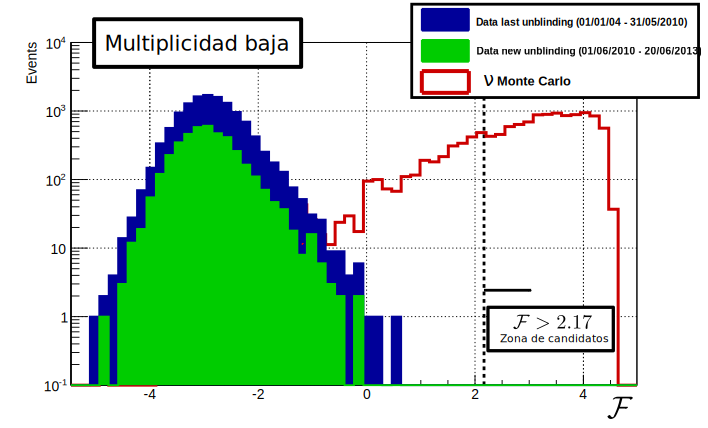
\includegraphics[width=0.85\textwidth]{fig/resultadosAuger/DGH_Retrining_May2012_2_low_Nor_mod}\\
			\caption{\label{fig:unblindingDGHL}
			Distribuci\'on de la variable de Fisher $\cal F$ para las muestras de b\'usqueda actual (verde) y pasada (azul) en eventos de multiplicidad baja. En rojo se muestra la distribuci\'on para la se\~nal simulada de neutrinos DGH.
			En l\'inea de trazos se muestra el corte de selecci\'on de candidatos.
			}
		\end{center}
	\end{figure}
	%
	\begin{figure}[ht!]
		\begin{center}
			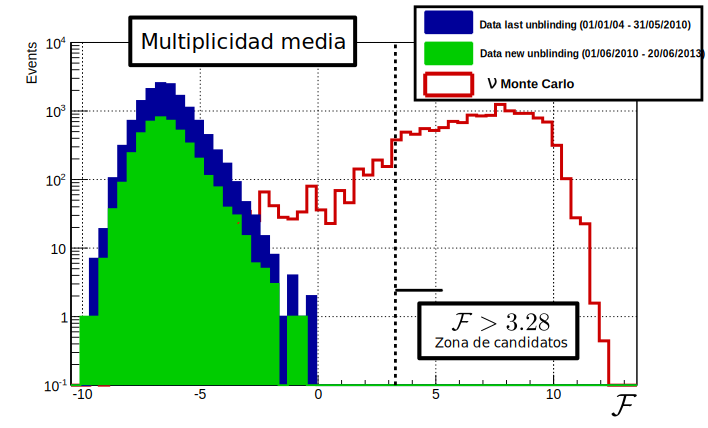
\includegraphics[width=0.85\textwidth]{fig/resultadosAuger/DGH_Retrining_May2012_2_med_Nor_mod}\\
			\caption{\label{fig:unblindingDGHM}
			Distribuci\'on de la variable de Fisher $\cal F$ para las muestras de b\'usqueda actual (verde) y pasada (azul) en eventos de multiplicidad media. En rojo se muestra la distribuci\'on para la se\~nal simulada de neutrinos DGH.
			En l\'inea de trazos se muestra el corte de selecci\'on de candidatos.
			}
		\end{center}
	\end{figure}
	%
	\begin{figure}[ht!]
		\begin{center}
			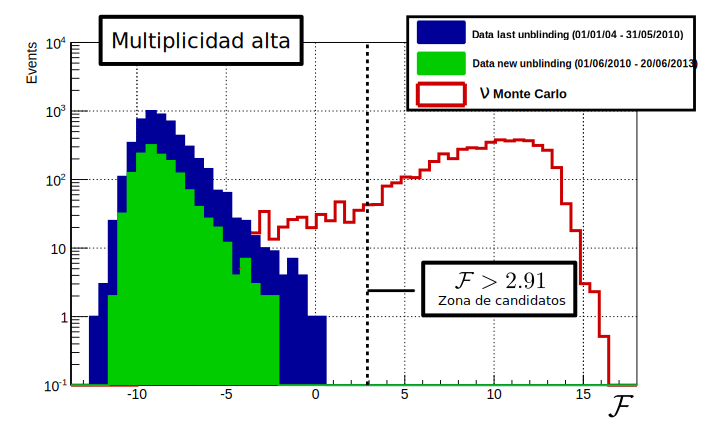
\includegraphics[width=0.85\textwidth]{fig/resultadosAuger/DGH_Retrining_May2012_2_high_Nor_mod}\\
			\caption{\label{fig:unblindingDGHH}
			Distribuci\'on de la variable de Fisher $\cal F$ para las muestras de b\'usqueda actual (verde) y pasada (azul) en eventos de multiplicidad alta. En rojo se muestra la distribuci\'on para la se\~nal simulada de neutrinos DGH.
			En l\'inea de trazos se muestra el corte de selecci\'on de candidatos.
			}
		\end{center}
	\end{figure}
	%
	\begin{figure}[ht!]
		\begin{center}
			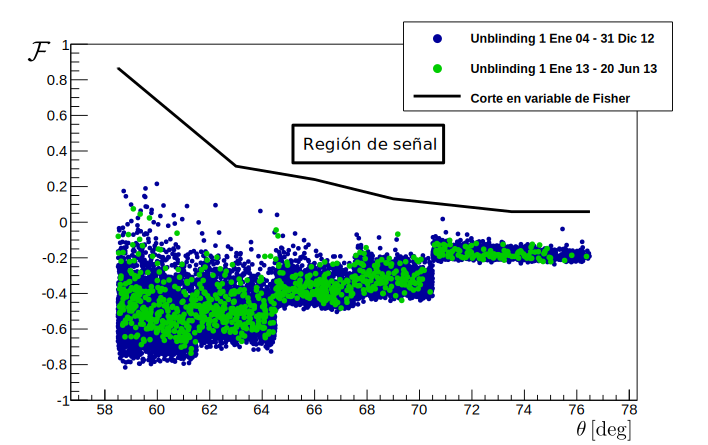
\includegraphics[width=0.85\textwidth]{fig/resultadosAuger/DGL_Unblinding_Thesis}\\
			\caption{\label{fig:unblindingDGL}
			Distribuci\'on de la variable de Fisher $\cal F$ para las muestras de b\'usqueda actual (verde) y pasada (azul) en funci\'on del \'angulo reconstruido. 
			%En rojo se muestra la distribuci\'on para la se\~nal simulada de neutrinos DGL.
			En l\'inea continua negra se muestra el corte de selecci\'on de candidatos.
			}
		\end{center}
	\end{figure}
	%
	
% 	\begin{figure}[ht!]
% 		\begin{center}
% 			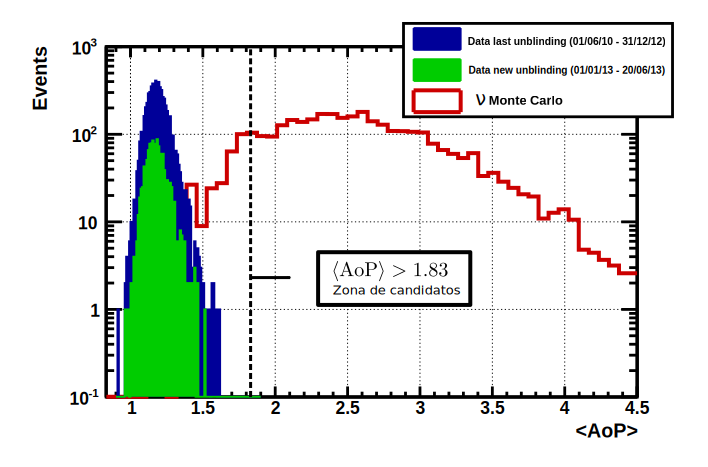
\includegraphics[width=0.7\textwidth]{fig/resultadosAuger/Unblinding_ES_200613}\\
% 			\includegraphics[width=0.7\textwidth]{fig/resultadosAuger/Unblinding_DGH_med_200613}\\
% 			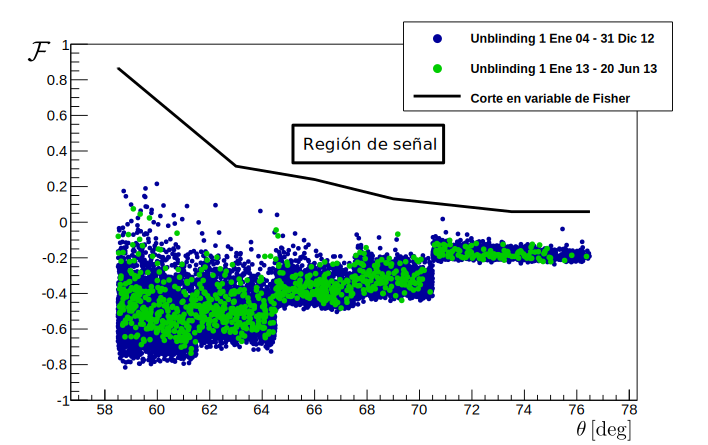
\includegraphics[width=0.7\textwidth]{fig/resultadosAuger/DGL_Unblinding_Thesis}
% 			\caption{Arriba: Distribuci\'on de las muestras de entrenamiento y b\'usqueda para la variable $\langle AoP \rangle$. En azul se muestra la distribuci\'on para la se\~nal simulada de neutrinos ES.
% 			Medio: Distribuci\'on de las muestras de entrenamiento y b\'usqueda para la variable de Fisher de la multiplicidad media. En azul se muestra la distribuci\'on para la se\~nal simulada de neutrinos DGH.
% 			Abajo: Variable de Fisher en funci\'on del \'angulo para las muestras de b\'usqueda correspondientes a las fechas 1 Enero 2004 - 31 Diciembre 2012 y 1 Enero 2013 - 20 Junio 2013.
% 			En los todos los gr\'aficos se muestra el corte de selecci\'on de candidatos, que no fue superado para ninguno de los tres an\'alisis.
% 			}
% 			\label{fig:unblindings}
% 		\end{center}
% 	\end{figure}
	
	\section{L\'imite al flujo difuso y diferencial}
	\label{sc:limiteAuger}
	Utilizando la exposici\'on combinada calculada en la secci\'on \ref{sc:expoNu}, y asumiendo un flujo diferencial de la forma $\Phi(E_\nu)= k\cdot E_\nu^{-2}$ y una relaci\'on entre sabores $\nu_e:\nu_\mu:\nu_\tau=1:1:1$, es posible obtener una cota superior al valor de $k$ mediante:
	%
	\begin{equation}
	 k_{up}=\frac{N_{up}}{\int\limits_{\mathbf{E_{\nu}}} E_\nu^{-2}\,{\cal E}_{Tot}(E_\nu) dE_\nu}
	 \label{eq:kup}
	\end{equation}
	%
	donde $N_{up}$ representa una cota superior a la cantidad de eventos esperados durante la medici\'on.
	Para obtener este valor se utiliz\'o la modificaci\'on al m\'etodo del cintur\'on de confianza para procesos poissonianos, desarrollado por Feldman y Cousins~\cite{cite:Feldman-Cousins}, y la extensi\'on semibayesiana de Conrad et al.~\cite{cite:Conrad_limit} que permite incorporar errores sistem\'aticos.
	En este m\'etodo, $N_{up}$ depende del n\'umero de eventos observado, del fondo esperado y del nivel de confianza elegido para la cota.
	Considerando que se observaron cero eventos, asumiendo de manera conservadora un fondo esperado despreciable, y requiriendo un nivel de confianza de \cant{90\%}{C.L.}, se obtiene $N_{up}=2.39$.
	Con este valor, y a partir de la ecuaci\'on \ref{eq:kup}, se calcul\'o una cota superior al flujo de neutrinos de
	%
	\begin{equation}
	k < 6.4 \times 10^{-9}~{\rm GeV~cm^{-2}~s^{-1}~sr^{-1}}.
	\label{eq:limitePosta}
	\end{equation}
	%
	Este l\'imite aplica en el rango \cant{1.0\times10^{17}}{eV} -- \cant{2.5\times10^{19}}{eV}, que es en el que se esperar\'ia detectar el \cant{90}{\%} de los eventos.
	Cabe destacar que este es el resultado m\'as estricto obtenido por el Observatorio Pierre Auger hasta la fecha, y el primero reportado como un \'unico l\'imite combinando la exposici\'on de los tres canales de detecci\'on.
	En la figura \ref{fig:intLimits} se muestra el límite obtenido junto al impuesto por IceCube y Anita-II, cada uno en su respectivo rango de energía.
	Tambi\'en se grafican los flujos predichos por distintos modelos de producci\'on cosmog\'enica.
	%
	\begin{figure}[ht!]
		\begin{center}
			\includegraphics[width=0.9\textwidth]{fig/resultadosAuger/integral_limits_and_models_paper_combined_proton}\\
			\includegraphics[width=0.9\textwidth]{fig/resultadosAuger/integral_limits_and_models_paper_combined_heavy}
			\caption{\label{fig:intLimits}
			L\'imite superior integral (a $90\%$C.L.) para el Observatorio Pierre Auger y para un flujo difuso de neutrinos calculado con un valor de $N_{up}=2.39$ (ver texto).
			Tambien se muestra el l\'imite alcanzado por ANITA\cite{cite:Anita2} y IceCube\cite{cite:IceCubePev} junto con los flujos esperados para varios modelos cosmog\'enicos\cite{Kampert_GZK,Ahlers_GZK,Kotera_GZK,Becker_AGN} y el l\'imite de Waxman-Bahcall\cite{cite:nuGRB}.}
		\end{center}
	\end{figure}
	
	Por otro lado, es posible integrar el denominador de la ecuaci\'on \ref{eq:kup} en intervalos de energ\'ia m\'as cortos, obteni\'endose as\'i un l\'imite superior $k_{up}$ en cada una, lo que se denomina un l\'imite diferencial. 
	El resultado se muestra en la figura \ref{fig:difLimits} para intervalos de energ\'ia de ancho 0.5 en escala $\log_{10}E_\nu$, junto al mismo l\'imite impuesto por IceCube y por ANITA-II.
	En el mismo gr\'afico se muestran distintos flujos cosmog\'enicos y la cota de Waxman-Bahcall.
	Este tipo de gr\'aficos permite comparar la sensitividad de distintos experimentos en cada rango de energ\'ia.
	Se observa que cerca de \cant{10^{18}}{eV}, la energ\'ia a la que los modelos predicen mayor afluencia de neutrinos, Auger es el experimento con mayor sensitividad.
	%
	\begin{figure}[ht!]
		\begin{center}
			\includegraphics[width=0.9\textwidth]{fig/resultadosAuger/diff_limits_and_models_paper_combined_all}
			\caption{\label{fig:difLimits}
			L\'imite superior diferencial (a $90\%$C.L. y bines de ancho 0.5 en $\log_{10}E_\nu$) para el Observatorio Pierre Auger y para un flujo difuso de neutrinos.
			Tambien se muestra el l\'imite alcanzado por ANITA\cite{cite:Anita2} y IceCube\cite{cite:IceCubePev} junto con los flujos esperados para varios modelos cosmog\'enicos\cite{Kotera_GZK,Kampert_GZK,Ahlers_GZK,Becker_AGN} y el l\'imite de Waxman-Bahcall\cite{cite:WaxmanBahcall1}.
			}
		\end{center}
	\end{figure}
	%
	
 	Finalmente, en la tabla \ref{tab:rates} se muestra el n\'umero total de eventos esperados para diferentes modelos de producci\'on de flujo de neutrinos.
 	Para obtener cada uno de estos valores se integr\'o la ecuaci\'on \ref{eq:expTot} utilizando el flujo correspondiente y la exposici\'on de la figura \ref{fig:expTot}.
 	%----------------------------------------------------------------------------------------
	\begin{table*}[!t]
	\begin{center}
	\renewcommand{\arraystretch}{1.3}
	\footnotesize
	\begin{tabular}{l c c} 
	\hline
	Modelo para       &  Número esperado de eventos     & ~Probabilidad de   \\
	el flujo difuso   &  (1 enero 2004 - 20 junio 2013) & ~observar $0$   \\
	\hline
	Cosmogénico - proton, FRII \cite{Kampert_GZK}     &  $\sim$ 4.0  & $\sim 1.8\times 10^{-2}$ \\

	Cosmogénico - proton, SFR \cite{Kampert_GZK}      &  $\sim$ 0.9  & $\sim 0.4$               \\

	Cosmogénico - proton, Fermi-LAT \cite{Ahlers_GZK} &  $\sim$ 3.2  & $\sim 4\times 10^{-2}$   \\

	Cosmogénico - band \cite{Kotera_GZK}              &  $\sim$ 0.5 $-$ 1.4 & $\sim 0.6~-~0.2$ \\

	Cosmogénico - iron, FRII \cite{Kampert_GZK}       &  $\sim$ 0.3  & $\sim 0.7$ \\

	\hline

	Astrofísico $\nu$ (AGN) \cite{Becker_AGN}     &  $\sim$ 7.2  & $\sim 7\times 10^{-4}$ \\

% 	\hline
% 
% 	Exótico \cite{Sigl}                               &  $\sim$ 31.5  & $\sim 2\times 10^{-14}$ \\

	\hline
	\end{tabular}
	\end{center}
	\vskip -3mm
	\caption{\label{tab:rates}
	Número esperado de eventos $N_{\rm esp}$ según la ecuación \ref{eq:expTot} para varios modelos teóricos de producción de neutrinos y para la exposición presentada en la figura \ref{fig:expTot}.
% 	Number of expected events $N_{\rm evt}$ in Eq.~(\ref{eq:Nevt}) for several theoretical models of UHE neutrino 
% 	production, given the combined exposure of the surface detector array
% 	of the Pierre Auger Observatory plotted in Fig.~\ref{fig:exposure}.
% 	The last column gives the Poisson probability $\exp({-N_{\rm evt}})$ of observing 0 events 
% 	when the number of expected events is $N_{\rm evt}$ given in the second column.
% 	% Kampert & Unger fluxes: Emax=Zx10^20 eV and alpha=2.0
	}
	\end{table*}
	
	A continuaci\'on se enumeran varias comentarios y conclusiones importantes:
	\begin{enumerate}
	 \item La sensitividad m\'axima del detector del SD de Auger se alcanza a energ\'ias alrededor del EeV, lo que coincide con el m\'aximo flujo esperado proveniente de modelos cosmog\'enicos.
	 \item El l\'imite actual de Auger es un factor cuatro veces m\'as chico que la cota superior de Waxman-Bahcall para la producci\'on de neutrinos en fuentes \'opticas, siendo el primer detector de rayos c\'osmicos en sobrepasar dicha cota.
	 \item Algunos modelos de producci\'on en fuentes astrof\'isicas, como AGN son excluidas con m\'as del \cant{90\%}{C.L.}
	 \item Los modelos cosmog\'enicos que asumen protones inyectados en la fuente como primarios y modelos de evoluci\'on fuertes (tipo FRII) se encuentran fuertemente desfavorecidos en las observaciones de Auger, aunque no pueden ser descartados hasta el momento.
	 \item Los modelos que proponen hierro como primarios o los menos optimistas entre los que suponen protones se encuentran por debajo del alcance del experimento, que necesitar\'ia ganar un factor 10 en exposici\'on para obtener resultados concluyentes.
% 	 \item Un gran n\'umero de modelos ex\'oticos son exluidos con \cant{99}{C.L.}.
% 	 \item 
	\end{enumerate}
	
\section{Comentarios finales de la primera parte}
	En los \'ultimos a\~nos se han detectado por primera vez neutrinos c\'osmicos de alta energ\'ia, sin embargo, hasta el momento su origen sigue siendo un misterio.
	La figura \ref{fig:multimess} muestra el estado actual de la detecci\'on, combinando el flujo medido en el ranglo del PeV por IceCube, los l\'imites diferenciales m\'as estrictos impuestos hasta el momento por Auger, IceCube, RICE y ANITA-II, y algunos flujos cosmog\'enicos.
	%
	\begin{figure}[ht]
		\begin{center}
		\includegraphics[width=0.75\textwidth]{fig/introduccion/1510-02050_multimessenger}
		\caption{\label{fig:multimess} Tomado de \cite{cite:multimess}. Flujo difuso de neutrinos medido por IceCube junto a los l\'imites impuestos por Auger, IceCube, Anita-II y Rice. Tambi\'en se muestran los flujos esperados para varios modelos cosmog\'enicos as\'i como la cota de Waxman-Bahcall.}
		\end{center}
	\end{figure}
	
	Tanto IceCube como Auger han alcanzado exposiciones sin precedentes, lo que ha permitido descartar los modelos de AGN y los cosmog\'enicos m\'as optimistas, mientras que el resto de los que suponen protones como primario comienzan a verse desfavorecidos.
	Por otro lado, los que utilizan una componente primaria m\'as pesada se encuentran todav\'ia lejos del alcance de la detecci\'on actual y por \'ultimo, una extrapolaci\'on del mejor ajuste del flujo medido por IceCube al rango de observaci\'on de Auger predice 0.1 eventos en su \'ultimo per\'iodo de medici\'on, compatible con una observaci\'on de 0 candidatos.
	
	Queda claro entonces que la nueva generaci\'on de detectores de neutrinos tiene mucho por descubrir.
	La observaci\'on del corte GZK respalda la existencia de un flujo cosmog\'enicos pero resultados recientes de Auger indican una migraci\'on hacia una componente m\'as pesada en los eventos de alta energ\'ia, lo que implicar\'ia flujos de neutrinos m\'as peque\~nos.
	Por este motivo la llegada de ARA, ARIANNA y GRAND generan mucha expectativa dentro de la comunidad.
	
	Siguiendo esta l\'inea, en la segunda parte de este trabajo se estudiar\'a el desempe\~no de un detector de superficie conformado por antenas de radio al detectar neutrinos c\'osmicos ultra energ\'eticos.
	
%----------------------------------------------------------------------------------------
	
% 	\begin{table}[ht!]
% 		\begin{center}
% 		\renewcommand{\arraystretch}{2.0}
% 			\begin{tabular}{|c|c|} 
% 			\hline
% 			Diffuse flux       &  Expected number of events   \\
% 			Neutrino Model     &  (1 Jan 04 - 20 Jun 13)   \\
% 			\hline
% 			\hline
% 			Cosmogenic (Kampert {\it et al.}) - proton, FRII      &  \textcolor{Red}{$\sim$ 4.0}  \\
% 			\hline
% 			Cosmogenic (Ahlers {\it et al.}) - proton, Fermi-LAT  &  \textcolor{Red}{$\sim$ 3.2}  \\
% 			\hline
% 			Cosmogenic (Kampert {\it et al.}) - proton, SFR       &  \textcolor{Blue}{$\sim$ 0.9}  \\
% 			\hline
% 			Cosmogenic (Kotera {\it et al.}) - band               &  \textcolor{Blue}{$\sim$ 0.5 $-$ 1.4}  \\
% 			\hline
% 			Cosmogenic (Kampert {\it et al.}) - iron, FRII        &  $\sim$ 0.3  \\
% 			\hline
% 			\end{tabular}
% 		\end{center}
% 	\end{table}
	

	
% 	\begin{figure}[ht!]
% 		\begin{center}
% 			\includegraphics[width=0.9\textwidth]{fig/resultadosAuger/diff_limits_and_many_models_IceCube_data_noextrap}
% 			\caption{asd}
% 			\label{fig:}
% 		\end{center}
% 	\end{figure}




	
	
	
% 	Al no encontrarse candidatos se procedió a fijar un límite al flujo de neutrinos. Usando la exposición~${\cal E}(E_{\nu})$ dada en la ecuación~\ref{eq:exposure}, la cantidad esperada de eventos~$N_{\rm esperado}$ para un flujo difuso de neutrinos $\Phi(E_{\nu})$ puede obtenerse por simple integración en energía:
% 	%
% 	\begin{equation}
% 	N_{\rm esperado}=\int_{E_{\rm min}}^{E_{\rm max}}\Phi(E_{\nu})\,{\cal E}(E_{\nu})\,{\rm d}E_{\nu}
% 	\label{eq:Nesp2}
% 	\end{equation}
% 	%
% 	Antes de que $N_{\rm esperado}$ pueda calcularse es necesario elegir una forma funcional para el flujo de neutrinos $\Phi$. Si para los tres sabores se asume un flujo diferencial típico de la forma $\Phi^{\nu_{\rm x}}=k^{\nu_{\rm x}}\cdot E_{\nu}^{-2}$ se tiene:
% 	%
% 	\begin{equation}
% 	N_{\rm esperado}^{\rm total} = N_{\rm esperado}^{\nu_{e}}+N_{\rm esperado}^{\nu_{\mu}}+N_{\rm esperado}^{\nu_{\tau}}
% 	\label{eq:Nesp3}
% 	\end{equation}
% 	%
% 	en donde cada uno de los $N_{\rm esperado}^{\nu_{\rm x}}$ puede escribirse como:
% 	%
% 	\begin{equation}
% 	N_{\rm esperado}^{\nu_{\rm x}}=k^{\nu_{\rm x}} \underbrace{\int_{E_{\rm min}}^{E_{\rm max}} E_{\nu}^{-2}\,{\cal E}^{\nu_{\rm X}}(E_{\nu})\,{\rm d}E_{\nu}}_{\equiv\,{\cal N}({\cal E}^{\nu_{\rm x}})} = k^{\nu_{\rm x}} \cdot {\cal N}({\cal E}^{\nu_{\rm x}})
% 	\label{eq:Nesp4}
% 	\end{equation}
% 	%
% 	la magnitud ${\cal N}({\cal E})$ tiene unidades de [GeV$^{-1}$~cm$^{2}$~s~sr] y solo depende de la exposición~${\cal E}$.
% 	Si se toma una relación 1:1:1 para los tres sabores ($k^{\nu_{e}}=k^{\nu_{\mu}}=k^{\nu_{\tau}}\equiv k$) consistente con el entendimiento actual sobre oscilaciones de neutrinos, la ecuación~\ref{eq:Nesp3} adquiere una forma más compacta:
% 	%
% 	\begin{equation}
% 	N_{\rm esperado}^{\rm total} = k \cdot ({\cal N}^{\nu_{e}} + {\cal N}^{\nu_{\mu}}+{\cal N}^{\nu_{\tau}}) = k \cdot{\cal N}^{\rm total}
% 	\label{eq:Nesp5}
% 	\end{equation}
% 	%
% 	Como veremos a continuación, esta expresión permite obtener un límite sobre la magnitud del flujo de cada sabor $k$.
% 
% 	Para explicar el método utilizado, es instructivo primero considerar un caso simplificado
% 	en que suponemos el fondo despreciable y la exposición ${\cal E}$ conocida sin error. El número $n$ de neutrinos observados es una variable aleatoria de distribución poissoniana $P_{\alpha}(n)$ con parámetro $\alpha$ igual a la cantidad de neutrinos esperada $N_{\rm esperado}^{\rm total}$ dada por~\ref{eq:Nesp5}. Si conociéramos $\alpha$, la probabilidad de observar al menos un neutrino está dada por
% 	$P_{\alpha}(n\geq1)=1-P_{\alpha}(0)$. A la inversa, sabiendo que el experimento no observó ningún neutrino, se define como rango estimado de $\alpha$ con un nivel de confianza (CL) de $p\times100\%$ al conjunto de valores que satisfacen $P_{\alpha}(n\geq1)< p$. Este conjunto es el intervalo $[0,\tilde\alpha]$ donde la cota superior $\tilde\alpha$ se obtiene de:
% 	%
% 	\begin{equation}
% 	P_{\tilde\alpha}(n\geq1)=p \Rightarrow 1-P_{\tilde\alpha}(0)=p \Rightarrow P_{\tilde\alpha}(0) = 1-p
% 	\end{equation}
% 	%
% 	En particular, la cota superior con un 90\% CL es:
% 	%
% 	\begin{equation}
% 	1-{\cal P}_{\tilde{\alpha}}(0) = 0.9 \Rightarrow 1-e^{\tilde{\alpha}} = 0.9 \Rightarrow \tilde{\alpha}\simeq2.3
% 	\label{eq:limite}
% 	\end{equation}
% 	% 
% 	Junto con la ecuación~\ref{eq:Nesp5} este resultado permite fijar una cota máxima para $k$ con un CL del 90\%:
% 	%
% 	\begin{equation}
% 	\left.
% 	\begin{array}{l}
% 	N_{\rm esperado}^{\rm total} = k \cdot{\cal N}^{\rm total} \\ \\
% 	N_{\rm esperado}^{\rm total} \leq 2.3
% 	\end{array}
% 	\right\}
% 	\Longrightarrow k \leq \frac{2.3}{{\cal N}^{\rm total}}
% 	\label{eq:limiteK}
% 	\end{equation}
% 	%
% 	Si se utiliza la exposición total dada en la Fig.~\ref{fig:exposure} se obtiene:
% 	%
% 	\begin{equation}
% 	k \leq 1.41 \times 10^{-7}~{\rm GeV~cm^{-2}~s^{-1}~sr^{-1}}
% 	\label{eq:limite2.3}
% 	\end{equation}
% 	%
% 	Es importante resaltar que este resultado se presenta solo a fines ilustrativos. El tratamiento simplificado utilizado, entre otras falencias, no incluye la predicción del fondo esperado ni la incerteza en la exposición.
% 
% 	Aunque el método anterior puede extenderse para incorporar el fondo~\cite{cite:Neyman}, tiene el problema de que no provee un marco unificado para el cálculo de límites superiores e inferiores (descubrimiento de un flujo).
% 	Con el fin de superar este inconveniente, Feldman y Cousins propusieron en~\cite{cite:Feldman-Cousins} una forma particular del método conocido como ``cinturón de confianza''~\cite{cite:cinturon} que implica, para el caso de un 90\% CL y un experimento sin fondo, reemplazar el 2.3 en~\ref{eq:limiteK} por 2.44. Si bien su esquema provee un marco unificado para el cálculo de límites (superiores e inferiores) con fondo, no incluye el tratamiento de las incertezas sistemáticas.
% 	Conrad y otros desarrollaron en~\cite{cite:Conrad_limit} una extensión semi Bayesiana del método que permite incorporar ésta información en el cálculo del límite. La idea es simple: a ${\cal N}$ y a $b$ se les asigna una distribución de probabilidad (PDF) que cuantifica la incerteza asociada a cada una de estas magnitudes~\footnote{Es la asignación de estas PDFs a priori la razón por la que el método es denominado ``semi Bayesiano".}. A continuación se promedia sobre todas las posibilidades y se obtiene un límite ``empeorado'' que incluye la incerteza en la eficiencia de identificación y el fondo.
% 
% 	Antes de poder aplicar el método es necesario entonces definir las PDFs que caracterizan a ${\cal N}$ y $b$.
% 	\begin{itemize}
% 	\item \textbf{PDF de la exposición:} la PDF de ${\cal N}$ está determinada por la incerteza en la exposición total. Tal como se discute en la Sec.~\ref{sec:erroresMC} se le puede asignar una distribución uniforme en el intervalo [-30\%,~+10\%]. 
% 	\item \textbf{PDF del fondo esperado:} a $b$ se le asignó una distribución gaussiana con un ancho dado por la propagación de la incerteza estadística en el modelo exponencial utilizado para describir la distribución de Fisher del fondo (ver Tab.~\ref{tab:bkgSysErr}). La incerteza sistemática proveniente de otras fuentes de fondo físico, como protones profundos, es despreciable.
% 	\end{itemize}
% 	%
% 	Es relevante destacar que el método no es muy sensible a la elección de la forma funcional de las distribuciones. Se obtienen resultados muy similares al utilizar gaussianas y uniformes de igual varianza.

	
